\section{Biểu diễn một chiều}
\begin{exercise}[3]
    Giải thích mối liên hệ giữa đặc trưng nhân tính và biểu diễn một chiều. Từ đó, diễn đạt lại bài toán phân loại các biểu diễn 1 chiều về bài toán đối với các đặc trưng nhân tính.
\end{exercise}
\begin{proof}
    Giả sử $V$ là một $K-$không gian vector 1 chiều và $G$ là một nhóm. 
    
    Vì $\varphi: K^* \to \GL(V),~\lambda \mapsto \lambda \Id_V$ là một đẳng cấu nhóm, nên với mỗi đặc trưng nhân tính của $G$
    \[\chi: G \to K^*\]
    cho ta một biểu diễn một chiều của $G$ trên $V$ là
    \[\rho = \varphi \circ \chi:G \to  \GL(V)\]
    và ngược lại mỗi biểu diễn một chiều $\rho$ cho ta một đặc trưng nhân tính của $G$
    \[\chi = \varphi^{-1}\circ \rho: G \to K^*.\]
    
    Vì vậy ta có đẳng cấu nhóm
    \[
        \Hom_{\mathrm{Rep}}(G, \GL(V)) \;\cong\; \Hom_{\mathrm{Grp}}(G, K^\ast).
    \]
    
Thật vậy,
\begin{itemize}
    \item Nếu $\rho : G \to \GL(V)$ là một biểu diễn, chọn một cơ sở $v_0$ của $V$.
    Khi đó, tồn tại $\lambda_g \in K^\ast$ sao cho $\rho(g)v_0 = \lambda_g v_0$.  
    Từ $\rho(gh) = \rho(g)\rho(h)$ suy ra $\lambda_{gh} = \lambda_g \lambda_h$,  
    nên ánh xạ $\chi_\rho : G \to K^\ast$, $\chi_\rho(g) = \lambda_g$, là một đồng cấu nhóm.

    \item Ngược lại, nếu $\chi : G \to K^\ast$ là một đặc trưng nhân tính, định nghĩa
\[
\rho_\chi(g)(v) = \chi(g)v, \quad \forall v \in V.
\]
Ta có $\rho_\chi(gh) = \rho_\chi(g)\rho_\chi(h)$, nên $\rho_\chi$ là một biểu diễn 1 chiều.  
    \item Hai ánh xạ $\rho \mapsto \chi_\rho$ và $\chi \mapsto \rho_\chi$ là nghịch đảo nhau, nên ta có
đẳng cấu nhóm
\[
\Hom_{\mathrm{Rep}}(G, \GL(V)) \cong \Hom_{\mathrm{Grp}}(G, K^\ast).
\]
\end{itemize}

Do đó, bài toán phân loại các biểu diễn một chiều của $G$ tương đương với bài toán phân loại các đặc trưng nhân tính, tức các đồng cấu nhóm $G \to K^\ast$. 
\end{proof}


\begin{exercise}[4]
    Cho $G$ là một nhóm. Cho $\chi$ là một đặc trưng nhân tính của nhóm $G$. Chứng minh rằng $\ker(\chi)$ chứa nhóm con giao hoán tử $[G,G]$ của $G$. Từ đó suy ra có tương ứng song ánh giữa tập hợp các đặc trưng nhân tính của nhóm $G$ và tập hợp các đặc trưng nhân tính của abel hoá $G^{ab}=G/[G,G]$ của nhóm $G$.
\end{exercise}
\begin{proof}
    Với mọi $[g,h] = ghg^{-1}h^{-1} \in [G,G]$ ta có
    \[\chi([g,h])= \chi(g)\chi(h)\chi(g^{-1})\chi(h^{-1})=\chi(g)\chi(h)\chi(g)^{-1}\chi(h)^{-1}=1\]
    nên $[G,G] \subseteq \ker(\chi)$.

    Hơn nữa $[G,G]$ là một nhóm con chuẩn tắc của $G$, vì $\forall x\in G,~\forall [g,h] \in [G,G]$ ta có
    \[a[g,h]a^{-1} = (aga^{-1})(aha^{-1})(ag^{-1}a^{-1})(ah^{-1}a^{-1}) \in [G,G].\]
    Do đó theo định lý đồng cấu nhóm, với mỗi đồng cấu nhóm (đặc trưng nhân tính) $\chi: G \to K^*$, tồn tại duy nhất $\overline{\chi}: G/[G,G] \to K^*$ sao cho $\chi =  \overline{\chi} \circ \pi$, với $\pi: G \to G/[G,G]$ là phép chiếu chính tắc.
    
    Do đó ta có một song ánh
    \[\Hom(G, K^*) \to \Hom(G^{ab}, K^*),~\chi \mapsto \overline{\chi}\]
    với ánh xạ ngược
    \[\Hom(G^{ab}, K^*) \to \Hom(G, K^*),~\varphi \mapsto \varphi \circ \pi\]
\end{proof}

\begin{exercise}[5]
    Tìm các đặc trưng nhân tính của nhóm cyclic. Lưu ý xét các trường hợp có thể xảy ra với trường $K$.
\end{exercise}
\begin{proof}
Giả sử $G$ là một nhóm cyclic, khi đó $G^{ab} = G$. Nên việc phân loại các đặc trưng nhân tính của $G$ quy về việc phân loại ảnh của phần tử sinh của $G$.

\begin{itemize}
  \item Nếu $G = \left<a\right> \cong \Z$ là một nhóm cyclic vô hạn. 
  
  Mỗi $\chi \in \Hom(G, K^*)$ được xác định duy nhất bởi ảnh của phần tử sinh $\lambda = \chi(a) \in K^*, ~\chi(a^k) = \lambda^k$.
  Khi đó $\Hom(G, K^*) \cong K^*,~ \chi \longleftrightarrow \chi(a)$.
  
  \item Nếu $G = \left<a\right> \cong \Z/n$ là một nhóm cyclic hữu hạn.
  
  Giả sử $\chi \in \Hom(G,K^*)$, khi đó $\chi(a)^n=1$. Tức là
  \[
  \chi(a) \in \mu_n(K)=\{x\in K^\times: x^n=1\}.
  \]
  Với mỗi $x\in\mu_n(K)$, đặt $\chi_x(a^m)=x^m$ ta được một đặc trưng nhân tính và mọi đặc trưng đều có dạng này. Vì thế
  \[
  \Hom(G,K^*) \cong\ \mu_n(K),\quad \chi \longleftrightarrow \chi(a) \in \mu_n(K).
  \]
  Xét các trường hợp cụ thể
  \begin{enumerate}
      \item Nếu $K$ là một trường đóng đại số và $\mathrm{char}(K)\nmid n$ thì $\mu_n(K) \cong \Z/n$ gồm các căn nguyên thủy bậc $n$ của 1. Nên có đúng $n$ đặc trưng nhân tính dạng $\chi(a) = \xi$ sao cho $\xi^n =1$.

      \item Nếu $K$ là một trường đóng đại số và $\mathrm{char}(K) = p \mid n$. Đặt $n = p^km$, với $\gcd(p,m)=1$, thì $\mu_n(K) = \mu_{m}(K) \cong \Z/m$ nên $\#\Hom(G,K^*) = |\mu_n(K)| = |\mu_m(K)|=m$.
  
    \item Nếu $K=\mathbb R$ thì $\mu_n(\mathbb R)$ bằng $\{1\}$ khi $n$ lẻ và bằng $\{ \pm1\}$ khi $n$ chẵn.
  
  \item Nếu $K=\mathbb F_q$, vì $\mathbb F_q^\times\cong \Z/(q-1)$ nên $\mu_n(\mathbb F_q)\cong \Z/\gcd(n,q-1)$.
  
  \end{enumerate}
\end{itemize}
\end{proof}

\begin{exercise}[6]
    Tìm các đặc trưng nhân tính của nhóm abel hữu hạn sinh. Lưu ý xét các trường hợp có thể xảy ra đối với trường $K$ (Sử dụng định lý phân loại nhóm abel hữu hạn sinh).
\end{exercise}
\begin{proof}
    Giả sử $G$ là một nhóm abel hữu hạn sinh. Theo định lý phân loại, tồn tại đẳng cấu
\[
G \cong \mathbb Z^{\,r}\ \oplus\ \bigoplus_{i=1}^t \Z/n_i,\qquad n_i\ge 2.
\]
Do đó
\[
\Hom(G,K^\times)\ \cong\ \Hom(\mathbb Z,K^\times)^{\,r}\ \times\ \prod_{i=1}^t \Hom(\Z/{n_i},K^\times)
\ \cong\ (K^\times)^{\,r}\ \times\ \prod_{i=1}^t \mu_{n_i}(K),
\]
trong đó $\mu_n(K)=\{a\in K^\times: a^n=1\}$ là nhóm nghiệm bậc $n$ của $X^n-1$ trong $K$.

Xét các trường hợp cụ thể cho trường $K$
\begin{enumerate}
    \item Nếu $K$ là một trường đóng đại số và $\mathrm{char}(K)\nmid n$ thì $\mu_n(K) \cong \Z/n$. Do đó
\[
\Hom(G,K^\times)\ \cong\ (K^\times)^{\,r}\times\prod_{i=1}^t \Z/{n_i}.
\]
      \item Nếu $K$ là một trường đóng đại số và $\mathrm{char}(K) = p \mid n$. Đặt $n = p^km$, với $\gcd(p,m)=1$, thì $\mu_n(K) = \mu_{m}(K) \cong \Z/m$. Do đó
      \[
\Hom(G,K^\times)\ \cong\ (K^\times)^{\,r}\times\prod_{i=1}^t \Z/{m_i}\quad \text{ với } m_i =\dfrac{n_i}{p^{v_p(n_i)}}
\]
  
    \item Nếu $K=\mathbb R$ thì $\mu_n(\mathbb R)$ bằng $\{1\} $ khi $n$ lẻ và bằng $\{ \pm1\}\cong \Z/2$ khi $n$ chẵn. Khi đó
  \[  \Hom(G,\mathbb R^\times)\ \cong\ (\mathbb R^\times)^{\,r}\times\prod_{i=1}^t \mu_{n_i}(\mathbb R),
\]
  
  \item Nếu $K=\mathbb F_q$, vì $\mathbb F_q^\times\cong \Z/(q-1)$ nên $\mu_n(\mathbb F_q)\cong \Z/\gcd(n,q-1)$.
    Do đó
\[
\Hom(G,\mathbb F_q^\times)\ \cong\ (\Z/(q-1))^{\,r}\times\prod_{i=1}^t \Z/{\gcd(n_i,q-1)},
\]
\[
\big|\Hom(G,\mathbb F_q^\times)\big|\ =\ (q-1)^{\,r}\ \prod_{i=1}^t\gcd(n_i,q-1).
\]
\end{enumerate}
\end{proof}

\begin{exercise}[7]
    Tính abel hoá của nhóm đối xứng $S_n$. Từ đó, xác định các đặc trưng nhân tính của nhóm đối xứng.
\end{exercise}
\begin{proof}
Với $n = 1$ hoặc $n=2$ thì $S_n$ là abel, nên $[S_n,S_n]=\{\Id\}$. Khi đó 
\[S_n^{ab} = S_n/[S_n,S_n] = S_n/\{\Id\} \cong S_n.\]

Với $n \geq 3$, ta sẽ chỉ ra $[S_n,S_n] = A_n$, khi đó 
\[S_n^{ab} = S_n/A_n = S_n/\ker(\sgn) \cong \im(\sgn) = \{\pm 1\} \cong \Z/2.\]
\begin{itemize}
    \item $[S_n, S_n] \subset A_n$. 
    
    Vì $\forall~[\sigma,\mu] = \sigma\mu\sigma^{-1}\mu^{-1} \in [S_n,S_n]$ thì $\sgn([\sigma,\mu])=1$.

    \item $A_n \subset [S_n, S_n]$.

    Mỗi phép thế trong $A_n$ là hợp thành của các xích độ dài 3. Thật vậy, mỗi phép thế $\sigma$ là hợp thành của một số chẵn các phép thế sơ cấp dạng $(a,b)$. Tính hợp thành từng cặp hai phép thế sơ cấp liên tiếp nói trên ta có hai trường hợp:
    \begin{itemize}
        \item Hai phép thế sơ cấp không rời nhau dạng $(a,b)(a,c) = (a,c,b)$.

        \item Hai phép thế sơ cấp rời nhau dạng $(a,b)(c,d)= (a,c,b)(a,c,d)$.
    \end{itemize}
    
    Mặt khác, mỗi phép thế độ dài 3 trong $A_n$ đều thuộc $[S_n,S_n]$. Thật vậy, với mỗi $\sigma = (a,b,c) \in A_n$, đặt $\tau = (a,c)$ thì 
    \[[S_n, S_n] \ni [\tau, \sigma] = \tau \sigma \tau^{-1}\sigma^{-1}= (\tau \sigma \tau)\sigma^{-1}=(\tau(a),\tau(b),\tau(c))\sigma^2 = (c,b,a)\sigma^2=\sigma^{-1}\sigma^2=\sigma.\]
\end{itemize}

\end{proof}

\begin{exercise}[8]
    Tính abel hoá của nhóm đối xứng $A_n$. Từ đó, xác định các đặc trưng nhân tính của nhóm thay phiên.
\end{exercise}
\begin{proof}
    Với $n = 1$ hoặc $n = 2$ thì $A_n = \{\Id\}$ nên $[A_n,A_n] = \{\Id\}$. Do đó $A_n^{ab} \cong 0$. 

    Với $n = 3$ thì $A_3 = \left<(1,2,3)\right> \cong  \Z/3$. Suy ra $[A_3, A_3] =  \{\Id\}$, và $A_3^{ab} \cong A_3 \cong \Z/3$.

    Với $n = 4$ thì $A_4$ gồm $\Id,$ các phép thế độ dài 3 dạng $(a,b,c)$ và các phép thế là tích của hai xích rời nhau độ dài 2 dạng $(a,b)(c,d) = (a,c,b)(a,c,d)$. 
    
    Ta có $V_4 = \{\Id, (1,2)(3,4),(1,3)(2,4), (1,4)(2,3)\}$ là một nhóm con của $A_4$. Hơn nữa còn là một nhóm con chuẩn tắc của $A_4$, vì $\forall \sigma \in A_4, \forall (a,b)(c,d) \in V_4$ ta có
    \[\sigma (a,b)(c,d)\sigma^{-1} = (\sigma (a,b)\sigma^{-1})(\sigma (c,d)\sigma^{-1})=(\sigma(a),\sigma(b))\,(\sigma(c),\sigma(d)) \in V_4.\]
    Vì thế nhóm thương $A_4/V_4 \cong \Z/3$ là một nhóm abel (vì $ |A_4/V_4| = 3$).

    Nhắc lại rằng, nếu $N \triangleleft G$ thoả mãn $G/N$ là abel thì $[G,G] \subset N$ (vì với $\pi_N: G \to G/N$ là phép chiếu chính tắc thì $\pi([x,y]) = \pi(xyx^{-1}y^{-1})=1$, do $G/N$ abel. Nên $[G,G] \subset \ker(\pi_N) = N$). Vì thế $[A_4,A_4] \subseteq V_4$.

    Mặt khác $V_4 \subseteq [A_4, A_4]$ vì $(a,b)(c,d)=[(a,b,c),(a,b,d)]$.

    Vì vậy $[A_4,A_4]= V_4$ và do đó $A_4^{ab} = A_4/V_4 \cong \Z/3$.
\end{proof}


\begin{exercise}[9]
    Tính abel hoá của nhóm nhị diện $D_n$. Từ đó, xác định các đặc trưng nhân tính của nhóm nhị diện.
\end{exercise}
\begin{proof}
    Ta có $D_n = \left<r,s: r^n = e,\, s^2 = e,\,srs^{-1} = r^{-1}\right>$ và
    \begin{itemize}
        \item $[r^i, r^j] = e = [s,s]$.

        \item $[s,r^i]^{-1}=[r^i,s] = r^isr^{-i}s^{-1}=r^i(sr^{n-i}s^{-1})=r^i(srs^{-1})^{n-i}=r^i(r^{-1})^{n-i}=r^{2i}$.

        \item $[s,r^is]^{-1} = [r^is,s] = r^isss^{-1}r^{-i}s^{-1} = r^i(sr^{n-i}s^{-1})=r^i(r^{-1})^{n-i}=r^{2i}$.
    \end{itemize}
    Vì thế $[D_n,D_n]  \subset \left<r^2\right>$. Mặt khác $r^2 = [r,s] \in [D_n,D_n]$ nên $\left<r^2\right> \subset [D_n,D_n]$.

    Vậy $[D_n, D_n] =  \left<r^2\right>$. Khi đó $D_n^{ab} = D_n/\left<r^2\right>$.
    \begin{itemize}
        \item Nếu $n$ lẻ thì $\left<r^2\right>=\left<r^{\gcd(2,n)}\right>=\left<r\right>$. Khi đó $|\left<r\right>| = n = |D_n|/2$. Vì thế $D_n^{ab} \cong \Z/2$ nếu $n$ lẻ.

        \item Nếu $n$ chẵn thì $|\left<r^2\right>| = n/2$ và do đó $|D_n^{ab}| = 4$. Tuy nhiên $D_n^{ab}$ không có phần tử cấp 4 vì $[r],[s]$ là các phần tử cấp 2 trong $D_n^{ab}$. Do đó với $n$ chẵn thì $D_n^{ab} \cong \Z/2 \times \Z/2$.
    \end{itemize}
    
\end{proof}

\begin{exercise}[10]
    Tính abel hoá của nhóm quaternion $Q_8$. Từ đó, xác định các đặc trưng nhân tính của nhóm $Q_8$.
\end{exercise}
\begin{proof}
    Ta có $Q_8 = \{\pm 1, \pm i, \pm j, \pm k\} = \left<i,j:i^2=j^2=k^2=ijk = -1\right>$ và
    \begin{itemize}
        \item $[i,j] = iji^{-1}j^{-1}=ij(-i)(-j)=ijij=k^2=-1$.

        \item $[j,k] = jkj^{-1}k^{-1}=jk(-j)(-k)=jkjk=i^2=-1$.

        \item $[k,i] = kik^{-1}i^{-1}=ki(-k)(-i)=kiki=j^2=-1$.

        \item $[i,i]=[j,j]=[k,k]=1$.
    \end{itemize}
    Do đó $[Q_8,Q_8]=\{\pm 1\}$. Vì thế $Q_8^{ab}=Q_8/\{\pm 1\} = \{\{\pm 1\}, i\{\pm 1\},j\{\pm 1\},k\{\pm 1\}\}$ có 3 phần tử cấp 2 và đơn vị $\{\pm 1\}$. Thế nên $Q_8^{ab}\cong \Z/2 \times \Z/2$.
\end{proof}

\begin{exercise}[11]
    Cho $\chi:G \to K^*$ là một đặc trưng nhân tính không tầm thường. Chứng minh rằng 
    \[\sum_{g \in G}\chi(g) = 0.\]
\end{exercise}
\begin{proof}
    Đặt $S = \sum_{g \in G}\chi(g)$. Vì $\chi$ không tầm thường nên tồn tại $x \in G$ để $\chi(x) \neq 1$. 
    
    Khi đó
    \[\chi(x)S=\sum_{g\in G}\chi(x)\chi(g)=\sum_{g\in G}\chi(xg) = \sum_{g'\in G}\chi(g') = S\]
    (vì $\{xG = G~\forall x\in G\}$).

    Suy ra $(\chi(x)-1)S = 0$, dẫn đến $S=0$, do $\chi(x)-1 \neq 0$.
\end{proof}


\section{Định nghĩa của biểu diễn nhóm}
\begin{exercise}[3]
    Cho $(\rho_1, V_1)$ và $\rho_2, V_2)$ là hai biểu diễn của nhóm $G$. Theo định nghĩa $\Hom_G(V_1, V_2)$ là một nhóm con của $\Hom_K(V_1, V_2)$. Tập con này có phải là một không gian con hay không? Vì sao?    
\end{exercise}
\begin{proof}
    Ta có 
    \[0 \in \Hom_G(V_1,V_2)=\{T \in \Hom_K(V_1,V_2): T\circ \rho_1(g) =  \rho_2(g)\circ T~\forall g\in G\} \subset \Hom_K(V_1,V_2)\]
    Hơn nữa, $\forall T,S \in \Hom_G(V_1,V_2),\forall \lambda,\mu \in K, \forall g\in G$ ta có $\lambda T +\mu S \in \Hom_G(V_1,V_2)$ vì 
    \[(\lambda T + \mu S)\rho_1(g) = \lambda T\rho_1(g)+\mu S\rho_2(g)=\lambda \rho_2(g)T+\mu\rho_2(g)S =  \rho_2(g)(\lambda T+\mu S). \]
    Do đó $\Hom_G(V_1,V_2)$ là một không gian vector con của $\Hom_K(V_1,V_2)$.
\end{proof}

\begin{exercise}[4]Hãy định nghĩa phạm trù $\Rep_K(G)$ của các biểu diễn $K$-tuyến tính của nhóm $G$. 
    
\end{exercise}
\begin{proof}
Định nghĩa phạm trù các biểu diễn $K$-tuyến tính của nhóm $G$, kí hiệu $\Rep_K(G)$ bởi 

\begin{enumerate}
  \item \textbf{Lớp các vật}
  \[
  \Ob(\Rep_K(G))
  = \{\, (\rho, V) \mid V \text{ là } K-\text{không gian vector trên}\; 
  \rho : G \to \GL(V) \text{ là đồng cấu nhóm} \,\}.
  \]
  Mỗi vật $(\rho,V)$ là một biểu diễn tuyến tính của $G$.

  \item \textbf{Lớp các cấu xạ}
  
  Với hai biểu diễn $(\rho_1,V_1)$ và $(\rho_2,V_2)$, đặt
  \[
  \Hom_G(V_1,V_2)
  = \{\, f \in \Hom_K(V_1,V_2)
  \mid f \circ \rho_1(g) = \rho_2(g) \circ f,\ \forall g \in G \,\}.
  \]
  
  Mỗi $f$ như vậy được gọi là một ánh xạ $G$-đồng cấu

  \item \textbf{Phép hợp thành các cấu xạ}
  
  Cho $f \in \Hom_G(V_1,V_2)$ và $g \in \Hom_G(V_2,V_3)$, định nghĩa
  \[
  g \circ f : V_1 \to V_3, \qquad (g \circ f)(v) = g(f(v)).
  \]
  Với mọi $h \in G, v\in V_1$ ta có
  \[
  (g \circ f)\rho_1(h)(v)
  = g(f(\rho_1(h)v))
  = g(\rho_2(h)f(v))
  = \rho_3(h)g(f(v))
  = \rho_3(h)(g \circ f)(v),
  \]
  nên $g \circ f \in \Hom_G(V_1,V_3)$.

  \item \textbf{Đồng nhất}
  Với mỗi vật $(\rho,V)$, cấu xạ đồng nhất là ánh xạ
  \[
  \Id_V : V \to V, \quad \Id_V(v)=v,
  \]
  hiển nhiên thoả $\Id_V \circ \rho(g)=\rho(g)\circ \Id_V$.

  \item \textbf{Tiên đề phạm trù:}
  \begin{itemize}
    \item (\emph{Tính kết hợp}) Với mọi $f : V_1 \to V_2$, $g : V_2 \to V_3$, $h : V_3 \to V_4$, ta có
    \[
    h \circ (g \circ f) = (h \circ g) \circ f.
    \]
    \item (\emph{Tính đồng nhất}) Với mọi $f : V_1 \to V_2$, ta có
    \[
    f \circ \Id_{V_1} = f = \Id_{V_2} \circ f.
    \]
  \end{itemize}
\end{enumerate}
Hơn nữa, vì mỗi $\Hom_G(V_1,V_2)$ là không gian vector trên $K$, nên $\Rep_K(G)$ còn là
một \emph{phạm trù $K$-tuyến tính}.
\end{proof}


\begin{exercise}[5]
    Chứng minh rằng phạm trù $\Rep_K(\Z/1\Z)$ đẳng cấu với phạm trù $\vect_K$. Như thế, một biểu diễn $K-$tuyến tính của nhóm một phần tử chính là một $K-$không gian vector. Trong trường hợp này, biểu diễn được phân loại dựa vào số chiều của nó.
\end{exercise}
% \begin{proof}
% Đặt $G=\Bbb Z/1\Bbb Z=\{e\}$ là nhóm tầm thường. Ta sẽ xây dựng một đẳng cấu phạm trù
% \[
% \Rep_K(G)\;\cong\;\vect_K .
% \]

% \textbf{(1) Mô tả vật và cấu xạ trong $\Rep_K(G)$.}
% Một vật của $\Rep_K(G)$ là một cặp $(\rho,V)$ với $V$ là $K$-không gian vector và
% $\rho:G\to\GL(V)$ là đồng cấu nhóm. Vì $G=\{e\}$, điều kiện đồng cấu buộc
% \[
% \rho(e)=\Id_V.
% \]
% Tức là \emph{mọi biểu diễn đều là tác động tầm thường} trên $V$, và do đó \emph{mỗi vật được xác định duy nhất bởi chính không gian $V$}.

% Với hai vật $(\rho_1,V_1),(\rho_2,V_2)$, một cấu xạ trong $\Rep_K(G)$ là ánh xạ $K$-tuyến tính
% $f:V_1\to V_2$ thỏa $f\circ\rho_1(e)=\rho_2(e)\circ f$. Nhưng $\rho_i(e)=\Id_{V_i}$, nên điều kiện này
% trở thành $f=f$, luôn đúng. Vì thế \emph{mọi ánh xạ $K$-tuyến tính $V_1\to V_2$ đều là cấu xạ trong $\Rep_K(G)$}.

% \textbf{(2) Hai hàm tử nghịch đảo.}
% Xét hai hàm tử
% \[
% F:\Rep_K(G)\longrightarrow\vect_K,\qquad F(\rho,V)=V,\quad F(f)=f,
% \]
% và
% \[
% G:\vect_K\longrightarrow\Rep_K(G),\qquad 
% G(V)=(\rho_{\mathrm{triv}},V)\ \text{ với }\ \rho_{\mathrm{triv}}(e)=\Id_V,\quad G(f)=f.
% \]
% Từ (1), $F$ và $G$ được xác định tốt trên vật và cấu xạ; rõ ràng chúng bảo toàn hợp thành và đồng nhất.

% \textbf{(3) Đẳng cấu phạm trù.}
% Ta có đẳng thức nghiêm ngặt trên hàm tử:
% \[
% F\circ G=\Id_{\vect_K},\qquad G\circ F=\Id_{\Rep_K(G)}.
% \]
% Thật vậy, với mọi $V$,
% $(F\circ G)(V)=F(\rho_{\mathrm{triv}},V)=V$, và với mọi $(\rho,V)$ (mà tất yếu $\rho=\rho_{\mathrm{triv}}$),
% $(G\circ F)(\rho,V)=G(V)=(\rho_{\mathrm{triv}},V)=(\rho,V)$.
% Tương tự trên cấu xạ, cả hai hợp đều là đồng nhất. Do đó $F$ và $G$ là hai nghịch đảo thực sự,
% suy ra $\Rep_K(G)\cong\vect_K$ là \emph{đẳng cấu phạm trù} (không chỉ tương đương).

% \textbf{(4) Hệ quả phân loại.}
% Vì các vật của $\Rep_K(G)$ chính là các $K$-không gian vector, nên lớp đẳng cấu của các biểu diễn
% (đặc biệt là hữu hạn chiều) được phân loại bởi \emph{số chiều}:
% \[
% (\rho,V)\ \simeq\ (\rho',V') \iff \dim_K V=\dim_K V'.
% \]
% Do định lý chọn cơ sở, với mỗi $n\in\Bbb N$ (và cả $n=\infty$ nếu xét vô hạn chiều) có đúng một lớp
% đẳng cấu biểu diễn bậc $n$.

% \end{proof}
% \begin{definition}[Hai phạm trù đẳng cấu]
% Hai phạm trù $\mathcal{C}$ và $\mathcal{D}$ được gọi là \textbf{đẳng cấu phạm trù}
% (nói ngắn gọn: \emph{đẳng cấu}) nếu tồn tại hai hàm tử
% \[
% F : \mathcal{C} \longrightarrow \mathcal{D}
% \quad\text{và}\quad
% G : \mathcal{D} \longrightarrow \mathcal{C}
% \]
% sao cho
% \[
% G \circ F = \Id_\mathcal{C}
% \quad\text{và}\quad
% F \circ G = \Id_\mathcal{D}.
% \]

% Tức là $F$ và $G$ là \emph{nghịch đảo đúng nghĩa của nhau}, cả trên vật lẫn trên cấu xạ.

% Biểu đồ tự nhiên mô tả điều này như sau:

% \[
% \begin{tikzcd}[column sep=huge, row sep=large]
% \mathcal{C}
%   \arrow[r, shift left=1.1ex, "F"]
% &
% \mathcal{D}
%   \arrow[l, shift left=1.1ex, "G"]
% \\
% \text{với } G \circ F = \Id_\mathcal{C},\;
% F \circ G = \Id_\mathcal{D}.
% \end{tikzcd}
% \]

% Nói cách khác, $F$ thiết lập một \textbf{song ánh hoàn toàn chính xác} giữa các vật và các cấu xạ:
% \[
% \begin{cases}
% \text{(i)} & \text{với mọi } X,Y \in \Ob(\mathcal{C}), \text{ ánh xạ } 
% \Hom_\mathcal{C}(X,Y) \xrightarrow{F} \Hom_\mathcal{D}(F(X),F(Y))
% \text{ là song ánh;} \\[4pt]
% \text{(ii)} & \text{với mọi } X \in \Ob(\mathcal{C}),\ G(F(X)) = X; \\
% \text{(iii)} & \text{với mọi } Y \in \Ob(\mathcal{D}),\ F(G(Y)) = Y.
% \end{cases}
% \]
% \end{definition}

\begin{proof}
Đặt $G = \mathbb{Z}/1\mathbb{Z} = \{ e \}$ là nhóm tầm thường. Ta chứng minh rằng
\[
\Rep_K(G) \;\cong\; \vect_K.
\]
\begin{enumerate}
    \item 

Lấy bất kỳ một vật $(\rho,V) \in \Ob(\Rep_K(G))$ khi đó 
\[
\rho : G \to \GL(V)
\]
là một đồng cấu nhóm. Vì $G = \{e\}$ nên $\rho(e) = \Id_V$.  
Do đó, mọi biểu diễn của $G$ là tác động tầm thường trên $V$, và vì vậy mỗi vật trong $\Ob(\Rep_K(G))$ được xác định duy nhất bởi chính không gian $V$. Nói cách khác ta có tương ứng $1-1$
\[\Rep_K(G) \ni (\rho,V) \longleftrightarrow V \in \vect_K\]


\item Giả sử $f \in \Hom_G(V_1,V_2)$ là một cấu xạ trong $\Rep_K(G)$, khi đó
\[
f \circ \rho_1(g) = \rho_2(g) \circ f, \quad \forall g \in G.
\]
Vì $\rho_i(e) = \Id_{V_i}$, điều kiện trên hiển nhiên đúng với mọi $f\in \Hom_K(V_1,V_2)$.  
Do đó:
\[
\Hom_G(V_1,V_2) = \Hom_K(V_1,V_2).
\]

Ta có biểu đồ giao hoán sau đúng với mọi $f$:
\[\begin{tikzcd}[ampersand replacement=\&,cramped]
	{V_1} \&\& {V_1} \\
	\\
	{V_2} \&\& {V_2}
	\arrow["{\rho_1(e)=\Id_{V_1}}", from=1-1, to=1-3]
	\arrow["f"', from=1-1, to=3-1]
	\arrow["f", from=1-3, to=3-3]
	\arrow["{\rho_2(e)=\Id_{V_2}}"', from=3-1, to=3-3]
\end{tikzcd}\]

\item Ta định nghĩa hai hàm tử

\[
F : \Rep_K(G) \longrightarrow \vect_K, \qquad
F(\rho,V) = V, \quad F(f) = f;
\]
\[
G : \vect_K \longrightarrow \Rep_K(G), \qquad
G(V) = (\rho_{\mathrm{triv}}, V), \quad G(f) = f,
\]
với $\rho_{\mathrm{triv}}(e) = \Id_V$.

Cả hai hàm tử này đều bảo toàn hợp thành và đồng nhất vì hợp thành của các ánh xạ tuyến tính không phụ thuộc vào cấu trúc nhóm.

Biểu đồ giao hoán
\[
\begin{tikzcd}
V_1 \arrow[r, "f"] \arrow[d, "\rho_{\mathrm{triv}}(e)=\Id_{V_1}"']
& V_2 \arrow[d, "\rho_{\mathrm{triv}}(e)=\Id_{V_2}"] \\
V_1 \arrow[r, "f"']
& V_2
\end{tikzcd}
\]
chứng tỏ $f$ là một $G-$đồng cấu trong mọi trường hợp.


\item Ta có:
\[
F \circ G = \Id_{\vect_K}, \qquad
G \circ F = \Id_{\Rep_K(G)}.
\]
Nói cách khác, biểu đồ dưới đây giao hoán cho mọi vật $(\rho,V)$:
\[
\begin{tikzcd}
(\rho,V) \arrow[r, "F"] \arrow[dr, "\Id"']
& V \arrow[d, "G"] \\
& (\rho_{\mathrm{triv}},V)
\end{tikzcd}
\]
Vậy $\Rep_K(G) \cong \vect_K$.
\end{enumerate}

\item Hơn nữa, vì các vật của $\Rep_K(G)$ tương ứng 1–1 với các $K$-không gian vector, nên hai biểu diễn
\[
(\rho,V),\ (\rho',V') \in \Rep_K(G)
\]
đẳng cấu khi và chỉ khi $V \cong V' \iff \dim_K V = \dim_K V'$.

Như vậy, các lớp đẳng cấu của biểu diễn của nhóm tầm thường được phân loại bởi số chiều:
\[
\Rep_K(G)\ \text{phân loại theo}\ \dim_K V.
\]

\end{proof}


\begin{exercise}[6]
    Xây dựng phạm trù $\mathcal{C}$ với vật là các cặp $(V,f)$ bao gồm một $K-$không gian vector $V$ và một tự đồng cấu $f: V \to V$ thoả mãn $f^n = \Id_V$. Sau đó, chứng minh rằng phạm trù $\mathcal{C}$ đẳng cấu với phạm trù $\Rep_K(\Z/n\Z)$. Như thế, một biểu diễn $K-$tuyến tính của nhóm $\Z/n\Z$ là một $K-$không gian vector trang bị một tự đồng cấu $f: V\to V$ thoả mãn $f^n = \Id_V$.
\end{exercise}
\begin{proof}
Đặt $G = \mathbb{Z}/n\mathbb{Z} = \langle [1] \rangle$.
Ta sẽ xây dựng một phạm trù $\mathcal{C}$ và chứng minh rằng
\[
\mathcal{C} \;\cong\; \Rep_K(G).
\]

\begin{enumerate}
    \item Định nghĩa phạm trù $\mathcal{C}$:
\begin{itemize}
  \item Lớp các vật: 
  \[\Ob(\mathcal{C}) = \{(V,f): V\in \Ob(\vect_K), f \in \Hom_K(V,V), f^n = \Id_V\}\]
  
  \item Lớp các cấu xạ:
  
  Một cấu xạ giữa hai vật $(V,f),~(W,g) \in \Ob(\mathcal{C})$ là một
  đồng cấu $K$-tuyến tính $\varphi:V\to W$ sao cho
  \[
  \varphi \circ f = g \circ \varphi.
  \]
  Hơn nữa, $\varphi\circ f^k = g^k\circ \varphi$. Thật vậy, giả sử khẳng định này đúng với $k = p$, khi đó
  \[\varphi \circ f^{p+1} =  (\varphi\circ f^p)\circ f=(g^p\circ \varphi)\circ f=g^p \circ (\varphi \circ f) = g^p \circ (g \circ \varphi) = g^{p+1}\circ \varphi.\]
  \item Hợp thành và đồng nhất:
  
  Lấy như trong phạm trù $\vect_K$,
  nghĩa là hợp thành của các đồng cấu tuyến tính và đồng nhất $\Id_V$.
\end{itemize}

Khi đó, ta có phạm trù
\[
\mathcal{C}
= \bigl( \Ob(\mathcal{C}),\ \Hom_\mathcal{C}(-,-),\ \circ,\ \Id \bigr).
\]

\item Xây dựng hàm tử giữa $\mathcal{C}$ và $\Rep_K(G)$
\[
F : \mathcal{C} \longrightarrow \Rep_K(G).
\]
\begin{itemize}
    \item Với mỗi $(V,f)\in \Ob(\mathcal{C})$, định nghĩa
\[
\rho : G \to \GL(V), \quad \rho([k]) = f^k.
\]

Ta thấy $\rho$ là một đồng cấu nhóm:
\[
\rho([k+l]) = f^{k+l} = f^k f^l = \rho([k])\rho([l]),
\]
và vì $f^n = \Id_V$ nên định nghĩa trên là tốt và do đó $F(V,f)=(\rho,V) \in \Rep_K(G)$.

\item Với $\varphi:(V,f)\to(W,g)$ trong $\mathcal{C}$, ta định nghĩa
\[
F(\varphi) = \varphi : V \to W.
\]
Khi đó $F(\varphi)\in\Hom_G(V,W)$ vì với mọi $k\in\mathbb{Z}$ ta có
\[
F(\varphi)\circ\rho_V([k])
= \varphi\circ f^k
= g^k\circ\varphi
= \rho_W([k])\circ F(\varphi).
\]

Như vậy $F$ xác định tốt trên cả vật lẫn cấu xạ, và bảo toàn hợp thành.

\[
\begin{tikzcd}[column sep=huge]
(V,f) \arrow[r, "F"] \arrow[d, "\varphi"']
& (\rho,V) \arrow[d, "F(\varphi)=\varphi"] \\
(W,g) \arrow[r, "F"]
& (\sigma,W)
\end{tikzcd}
\quad
\text{với } \rho([k])=f^k,\; \sigma([k])=g^k.
\]
\end{itemize}
\item Định nghĩa hàm tử nghịch đảo của $F$
\[
F' : \Rep_K(G) \longrightarrow \mathcal{C}.
\]

\begin{itemize}
    \item Với mỗi vật $(\rho,V)\in\Rep_K(G)$, đặt
\[
f = \rho([1]) \in \GL(V).
\]
Ta có $\rho([n]) = \rho([0]) = \Id_V$, nên
\[
f^n = \rho([1])^n = \rho([n]) = \Id_V.
\]
Vậy $(V,f)=F'(\rho,V)\in \Ob(\mathcal{C})$.

\item Với mỗi $G$-đồng cấu $\psi:(\rho_1,V_1)\to(\rho_2,V_2)$, ta định nghĩa
\[
F'(\psi)=\psi:V_1\to V_2.
\]
Ta có
\[
\psi\circ\rho_1([k])=\rho_2([k])\circ\psi
\]
nói riêng khi $k=1$, đặt $f_i = \rho_i([1])$ ta được
\[
\psi\circ f_1 = f_2\circ\psi,
\]
Dẫn đến $F'(\psi)=\psi \in \Hom_{\mathcal{C}}((V_1,f_1),(V_2,f_2))$.
\end{itemize}

\item
Trước hết, với $(V,f)\in\mathcal{C}$, vì $\rho([1])=f$ nên
\[
(F'\circ F)(V,f)
= F'(\rho,V)
= (V,\rho([1]))
= (V,f),
\]
Ngược lại, với $(\rho,V)\in\Rep_K(G)$,
\[
(F\circ F')(\rho,V)
= F(V,f=\rho([1]))
= (\rho',V),
\]
trong đó $\rho'([k])=f^k=\rho([1])^k=\rho([k])$,
nên $(\rho',V)=(\rho,V)$.

Hay nói cách khác
\[
F\circ F' = \Id_{\Rep_K(G)}, \quad F'\circ F = \Id_{\mathcal{C}}.
\]
\item Vậy
\[
\mathcal{C} \;\cong\; \Rep_K(\mathbb{Z}/n\mathbb{Z})
\]

Nói cách khác, \emph{một biểu diễn $K$-tuyến tính của nhóm $\mathbb{Z}/n\mathbb{Z}$ chính là một $K$-không gian vector $V$ cùng với một tự đồng cấu $f:V\to V$ sao cho $f^n=\Id_V$.}
\end{enumerate}
\end{proof}


\begin{exercise}[7]
    Một tự đồng cấu tuyến tính $f: V\to V$ thoả mãn $f^2 =  \Id_V$ được gọi là một tự đồng cấu \textbf{đối hợp}. Ta có thể nói gì về những tự đồng cấu này? Chúng có chéo hoá được hay không? Hãy phân loại các tự đồng cấu đối hợp, từ đó, phân loại các biểu diễn của nhóm $\Z/2\Z$. 
\end{exercise}
\begin{proof}
Mỗi tự đồng cấu tuyến tính $f:V\to V$ thoả $f^2=\Id_V$ (được gọi là \emph{đối hợp}) thì $f$ khả nghịch với $f^{-1}=f$ và mọi trị riêng $\lambda$ thoả $\lambda^2=1$, tức $\lambda \in \{\pm 1 \}$. Hơn nữa, đa thức tối tiểu của $f$ là $m_f(x) \mid (x-1)(x+1)$.

\begin{enumerate}
    \item Nếu $\operatorname{char}K\ne2$.
    
    Khi đó $m_f(x) = (x-1)(x+1)$ tách được trên $K$, do đó $f$ chéo hoá được. Cụ thể
\[
V=V_+\oplus V_-,\qquad 
V_\pm=\ker(f\mp\Id_V),
\]
Đặt $r =  \dim V_+,~s =  \dim V_{-}$, chọn một cơ sở thích hợp ta thu được ma trận biểu diễn của $f$ là
\[
[f]=\begin{pmatrix} I_r & 0\\ 0 & -I_s\end{pmatrix}.
\]
Do đó hai đối hợp đẳng cấu khi và chỉ khi cùng cặp số $(r,s)$.
Biểu diễn tương ứng của $\Z/2\Z$ là 
\[
\rho([1])=f,\quad f^2=\Id_V,
\]
Do $\Z/2\Z$ có hai biểu diễn một chiều
\[
\chi_+([1])=1,\qquad \chi_-([1])=-1,
\]
Ta sẽ chỉ ra mọi biểu diễn hữu hạn chiều phân rã thành
\[
V \cong K_+^{\oplus r} \oplus K_-^{\oplus s}.
\]
với $K_\pm$ là hai biểu diễn một chiều: $[1]\mapsto\pm1$.

Thật vậy, ký hiệu $K_+=(K,\rho_+)$ với $\rho_+([1])=+1$, và $K_-=(K,\rho_-)$ với $\rho_-([1])=-1$.
Đây là hai biểu diễn 1 chiều của $\Bbb Z/2\Bbb Z$.

Chọn cơ sở riêng $\{e_1,\dots,e_r\}$ của $V_+$ và $\{f_1,\dots,f_s\}$ của $V_-$.

Khi đó, với mọi $i$, ta có $f(e_i)=+e_i$ và $f(f_j)=-f_j$.

Xét không gian
\[
K_+^{\oplus r}\oplus K_-^{\oplus s}
\;=\;
\underbrace{K_+\oplus\cdots\oplus K_+}_{r\ \text{lần}}
\ \oplus\
\underbrace{K_-\oplus\cdots\oplus K_-}_{s\ \text{lần}}.
\]
Một phần tử ở vế trái có dạng
\[
(\alpha_1,\dots,\alpha_r;\ \beta_1,\dots,\beta_s),\quad \alpha_i,\beta_j\in K,
\]
trong đó $[1]$ tác động bằng
\[
[1]\cdot(\alpha_1,\dots,\alpha_r;\ \beta_1,\dots,\beta_s)
=(\alpha_1,\dots,\alpha_r;\ -\beta_1,\dots,-\beta_s).
\]
Định nghĩa ánh xạ tuyến tính
\[
\Phi:\ K_+^{\oplus r}\oplus K_-^{\oplus s}\ \longrightarrow\ V,\qquad
\Phi(\alpha,\beta)\ =\ \sum_{i=1}^r \alpha_i e_i\ +\ \sum_{j=1}^s \beta_j f_j.
\]
$\Phi$ là một ánh xạ tuyến tính, hơn nữa là một đẳng cấu (vì $\{e_i\}\cup\{f_j\}$ là cơ sở của $V$).

Mặt khác, $\Phi$ cũng là một \emph{$G$-đồng cấu} vì
\[
\Phi\big([1]\cdot(\alpha,\beta)\big)
= \sum_i \alpha_i e_i\ -\ \sum_j \beta_j f_j
= f\!\left(\sum_i \alpha_i e_i+\sum_j \beta_j f_j\right)
= f\big(\Phi(\alpha,\beta)\big)
= [1]\cdot\Phi(\alpha,\beta).
\]
Vì vậy, $\Phi$ là đẳng cấu biểu diễn, vì thế
\[
V\ \cong \ K_+^{\oplus r}\ \oplus\ K_-^{\oplus s}.
\]

\item Nếu $\operatorname{char}K = 2$.

Khi đó $1 = -1$ trong $K$, nên $m_f(x) \mid (x - 1)^2$.

\begin{itemize}
  \item Nếu $m_f(x) = x - 1$, thì $f = \Id_V$, hiển nhiên chéo hoá được.

  \item Nếu $m_f(x) = (x - 1)^2$, thì $f$ không chéo hoá được. Khi đó ta đặt
  \[
  N := f - \Id_V.
  \]
  Suy ra $N$ là toán tử nilpotent cấp 2, tức $N^2 = 0$, và $f = \Id_V + N$.
  Toán tử $N$ có thể khác 0, nhưng thoả $N^2=0$ nên dạng Jordan của $N$ chỉ gồm các khối Jordan nilpotent cỡ $1$ hoặc $2$:
  \[
  J_1(0) = (0), \qquad J_2(0) =
  \begin{pmatrix}
  0 & 1 \\ 0 & 0
  \end{pmatrix}.
  \]
  Khi đó dạng Jordan của $f = \Id_V + N$ thu được bằng cách cộng $1$ vào mỗi giá trị riêng của $N$, tức là:
  \[
  J_1(1) = (1), \qquad
  J_2(1) =
  \begin{pmatrix}
  1 & 1 \\ 0 & 1
  \end{pmatrix}.
  \]
\end{itemize}

Vì vậy
\[
\Rep_K(\Z/2\Z)
\simeq
\{(V,f)\mid f^2=\Id_V\},
\]
với
\[
f\sim
\begin{cases}
\mathrm{diag}(I_r,-I_s), & \text{nếu }\operatorname{char}K\ne2,\\[3pt]
\Id_V+N,\ N^2=0, & \text{nếu }\operatorname{char}K=2.
\end{cases}
\]
Trong trường hợp $\operatorname{char}K\ne2$, các biểu diễn được phân loại bởi cặp số $(r,s)$,
còn khi $\operatorname{char}K=2$, chúng được phân loại theo dạng Jordan của $f$, tức là bởi số lượng
khối $J_1(1)$ và $J_2(1)$.
\end{enumerate}
\end{proof}


\begin{exercise}[8]
    Cho $n \geq 2$ là một số nguyên dương cố định. Ta có thể nói gì về cấu trúc của tự đồng cấu tuyến tính $f: V \to V$ thoả mãn $f^n =  \Id_V$. Có thể sử dụng những thông tin này để phân loại các biểu diễn của nhóm $\Z/n\Z$ như thế nào?
\end{exercise}
\begin{proof}
Giả sử $K$ là một trường và $n\ge2$ là số nguyên dương cố định.  

Vì $\Rep_K(\Z/n\Z)
\;\simeq\;
\{(V,f)\mid f^n=\Id_V\}$ nên mọi biểu diễn hữu hạn chiều $(\rho,V)$ của $\Z/n\Z$ trên $K$ được xác định bởi $f := \rho([1]) \in \GL(V),$ thỏa mãn $f^n=\Id_V$.  
Ngược lại, mọi $f\in\GL(V)$ thoả $f^n=\Id_V$ xác định một biểu diễn của $\Z/n\Z$ qua
$\rho([k])=f^k$.

Ta phân loại các biểu diễn này theo cấu trúc của toán tử $f$.

\begin{enumerate}
\item \textbf{Trường hợp $K$ chứa đầy đủ các căn bậc $n$ của đơn vị và $\operatorname{char}K\nmid n$.}

Khi đó đa thức $x^n-1$ tách hoàn toàn và có $n$ nghiệm phân biệt:
\[
x^n-1 = \prod_{j=0}^{n-1} (x - \zeta_n^j),
\]
với $\zeta_n$ là căn nguyên thủy bậc $n$.  
Từ $f^n=\Id$ suy ra đa thức tối tiểu $m_f(x)\mid (x^n-1)$, nên $f$ chéo hoá được.  
Tồn tại phân rã
\[
V = \bigoplus_{\lambda^n=1} V_\lambda,
\qquad
V_\lambda := \ker(f - \lambda\Id_V),
\]
với mỗi $V_\lambda$ là không gian riêng ứng với trị riêng $\lambda$ (căn bậc $n$ của 1).  

Trên $V_\lambda$, $\Z/n\Z$ tác động qua biểu diễn 1 chiều:
\[
K_\lambda :\quad \rho_\lambda([1])=\lambda.
\]
Suy ra
\[
V \cong \bigoplus_{\lambda^n=1} K_\lambda^{\oplus r_\lambda},
\qquad r_\lambda = \dim V_\lambda.
\]
% \emph{Phân loại:} bởi các số nguyên không âm $(r_\lambda)_{\lambda^n=1}$.  
% Đây là trường hợp đơn giản và “đẹp nhất”: mọi biểu diễn đều chéo hoá được và là tổng của các biểu diễn 1 chiều.

\item \textbf{Trường hợp $\operatorname{char}K\nmid n$ nhưng $K$ không chứa đủ các căn bậc $n$ của đơn vị.}

Lúc này $x^n-1$ tách thành tích của các đa thức bất khả quy trên $K$:
\[
x^n-1 = p_1(x)p_2(x)\cdots p_t(x),
\quad p_i(x)\in K[x]\ \text{bất khả quy và phân biệt.}
\]
Từ $f^n=\Id$ suy ra $m_f(x)\mid (x^n-1)$, nên tồn tại phân rã sơ cấp
\[
V = \bigoplus_{i=1}^t V_{p_i},
\qquad V_{p_i} := \ker(p_i(f)).
\]
Trên mỗi $V_{p_i}$, toán tử $f$ có đa thức tối tiểu $p_i(x)^k$ cho một số $k\ge1$.  
Nếu $k=1$, $f$ chéo hoá trên $V_{p_i}$; nếu $k>1$, $f$ có khối Jordan tương ứng.  

% \emph{Phân loại:} bởi dạng Jordan của $f$ tương ứng với các đa thức bất khả quy $p_i(x)$ của $x^n-1$.  
% Mỗi $p_i$ tương ứng với một “loại” biểu diễn con (biểu diễn 1D khi $p_i$ tuyến tính, và biểu diễn nhiều chiều khi $p_i$ bậc cao hơn).

\medskip
\item \textbf{Trường hợp $\operatorname{char}K\mid n$.}

Khi đó $x^n-1$ có nghiệm kép tại $x=1$, vì đạo hàm $(x^n-1)' = n x^{n-1} \equiv 0$.
Ta có
\[
x^n - 1 = (x - 1)^n.
\]
Từ $f^n = \Id$ suy ra $(f-\Id)^n = 0$.  
Đặt $N := f - \Id$, thì $N$ là toán tử nilpotent với $N^n=0$, nên
\[
f = \Id + N.
\]
Dạng Jordan của $f$ chỉ gồm các khối Jordan ở trị riêng $1$ là $J_k(1)$

Ta phân loại chúng bởi số lượng các khối Jordan $J_k(1)$ của $f$.
\end{enumerate}

\end{proof}

\begin{exercise}[9]
    Tương tự những bài tập trên, hãy xem xét các biểu diễn $K-$tuyến tính của nhóm $\Z$.
\end{exercise}
\begin{proof}
    % Biểu diễn của $\Z$ là cặp $(V,f)$ với $f\in\GL(V)$
Xét phạm trù $\mathcal C$ với
\[
\Ob(\mathcal C)=\{(V,f)\mid V\text{ là }K\text{-không gian vector, } f\in\GL(V)\}\]
\[
\Hom_{\mathcal C}\big((V,f),(W,g)\big)=\{\varphi:V\to W\mid \varphi f=g\varphi\}.
\]
Khi đó có đẳng cấu phạm trù
\[
\Rep_K(\Z)\ \cong\ \mathcal C.
\]
% Nhắc rằng $\Z=\langle 1\rangle$ là nhóm sinh bởi $1$ với \emph{không có quan hệ hữu hạn} nào (ngoài đơn vị).
Do đó một biểu diễn $(\rho,V)$ của $\Z$ được xác định duy nhất bởi $f:=\rho(1)\in\GL(V)$, và
\[
\rho(k)=\rho(1)^k=f^k\quad (\forall k\in\Z).
\]

Ta xây dựng hàm tử giữa chúng
\begin{enumerate}
    \item $F:\mathcal C\to\Rep_K(\Z)$.
    \begin{itemize}
    \item Trên vật, đặt
\[
F(V,f)=(\rho_f,V),\qquad \rho_f(k):=f^k\in\GL(V).
\]
Vì $f$ khả nghịch, $f^k$ xác định tốt với mọi $k\in\Z$, và $\rho_f(k+\ell)=f^{k+\ell}=f^kf^\ell$ nên $\rho_f$ là đồng cấu nhóm.

    \item Trên cấu xạ, nếu $\varphi:(V,f)\to(W,g)$ với $\varphi f=g\varphi$, thì với mọi $k\in\Z$ ta có
\[
\varphi\circ\rho_f(k)=\varphi f^k=g^k\varphi=\rho_g(k)\circ\varphi,
\]
nên $F(\varphi)=\varphi$ là $G$-tuyến tính. Do đó $F$ là một hàm tử.
\end{itemize}

\item $G:\Rep_K(\Z)\to\mathcal C$.

Trên vật, đặt
\[
G(\rho,V)=(V,f:=\rho(1)).
\]
Vì $\rho(1)\in\GL(V)$ nên $f$ khả nghịch. Trên cấu xạ, nếu $\psi:(\rho_1,V_1)\to(\rho_2,V_2)$ là $G$-đồng cấu, với $1\in\Z$:
\[
\psi\circ \rho_1(1)=\rho_2(1)\circ\psi \quad\Longleftrightarrow\quad \psi f_1=f_2\psi,
\]
nên $G(\psi)=\psi$ là cấu xạ trong $\mathcal C$.

\item $F$ và $G$ là nghịch đảo của nhau.

Với $(\rho,V)\in\Rep_K(\Z)$, ta có
\[
(F\circ G)(\rho,V)=F(V,\rho(1))=(\rho',V),\quad \rho'(k)=\rho(1)^k=\rho(k),
\]
nên $(F\circ G)=\Id_{\Rep_K(\Z)}$ (cả trên vật lẫn cấu xạ).
Với $(V,f)\in\Ob(\mathcal C)$,
\[
(G\circ F)(V,f)=G(\rho_f,V)=(V,\rho_f(1))=(V,f),
\]
nên $(G\circ F)=\Id_{\mathcal C}$.
Suy ra $F$ và $G$ là hai nghịch đảo phạm trù, do đó $\Rep_K(\Z)\cong\mathcal C$.
\end{enumerate}
% \begin{theorem}[Phân loại các biểu diễn $K$-tuyến tính của $\Z$]

Vậy mọi biểu diễn hữu hạn chiều $(\rho,V)$ của nhóm $\Z$ trên trường $K$
được xác định duy nhất bởi một tự đẳng cấu tuyến tính $f = \rho(1) \in \GL(V)$,
với $\rho(k) = f^k$.
Do đó,
\[
\Rep_K(\Z) \simeq \{(V,f)\mid f \in \GL(V)\}.
\]
Hai biểu diễn $(\rho_1,V_1)$ và $(\rho_2,V_2)$ đẳng cấu khi và chỉ khi
hai toán tử tương ứng $f_1 = \rho_1(1)$ và $f_2 = \rho_2(1)$ đồng dạng.
Khi đó, việc phân loại các biểu diễn của $\Z$ tương đương với việc phân loại
các ma trận khả nghịch trong $\GL_n(K)$ theo dạng chuẩn Jordan.

\begin{enumerate}[label=\textnormal{(\roman*)}]
\item \textbf{Nếu $K$ đóng đại số}

Tồn tại một cơ sở của $V$ sao cho sao cho
\[
f \sim \bigoplus_{i=1}^t J_{m_i}(\lambda_i),
\]
% với $\lambda_i \in K^\times$ và
% \[
% J_{m}(\lambda) =
% \begin{pmatrix}
% \lambda & 1 & 0 & \cdots & 0\\
% 0 & \lambda & 1 & \ddots & \vdots\\
% \vdots & & \ddots & \ddots & 0\\
% 0 & \cdots & 0 & \lambda & 1\\
% 0 & \cdots & \cdots & 0 & \lambda
% \end{pmatrix}.
% \]
Vì $f$ khả nghịch nên mọi $\lambda_i \ne 0$.
Do đó, mọi biểu diễn hữu hạn chiều của $\Z$ được phân loại bởi đa tập các cặp $(\lambda,m)$, trong đó: $\lambda \in K^\times$ là trị riêng của $f$ và $m$ là kích thước của khối Jordan tương ứng.

Nếu $f$ chéo hoá được (tức mọi khối đều có $m=1$), ta có
\[
V \simeq \bigoplus_{\lambda\in K^\times} K_\lambda^{\oplus r_\lambda},
\qquad K_\lambda:\ 1\mapsto\lambda,
\]
với $r_\lambda = \dim V_\lambda$.
Các biểu diễn 1 chiều của $\Z$ chính là
\[
\Hom(\Z, K^\times) \simeq K^\times,\qquad
\rho_\lambda(1)=\lambda.
\]

% \item 
% Cho $(\rho,V)$ là một biểu diễn hữu hạn chiều của $\Z$ trên $K$, đặt $f=\rho(1)\in\GL(V)$.
% Khi đó tồn tại các đa thức bất khả quy đôi một khác nhau $p_1,\dots,p_s\in K[x]$
% và các số mũ $m_{i1}\ge m_{i2}\ge\cdots\ge m_{i\ell_i}\ge1$ sao cho
% \[
% V \;\cong\; \bigoplus_{i=1}^s \bigoplus_{j=1}^{\ell_i} K[x]_{p_i^{\,m_{ij}}},
% \qquad
% K[x]_{p^m} := K[x]/(p(x)^m),
% \]
% với tác động của $f$ là phép nhân bởi lớp $x$.
% Tương đương, với một cơ sở thích hợp ta có dạng hữu tỉ (rational canonical form):
% \[
% f \;\sim\; \bigoplus_{i=1}^s\ \bigoplus_{j=1}^{\ell_i}
% C\!\left(p_i(x)^{\,m_{ij}}\right),
% \]
% trong đó $C(q)$ là ma trận bạn đồng hành (companion matrix) của đa thức $q$.


% \begin{proof}[Phác thảo]
% Xem $V$ như một $K[x]$-môđun với $x$ tác động bởi $f$. Theo định lý cấu trúc môđun
% trên PID $K[x]$, ta có phân rã theo \emph{thừa số sơ cấp}:
% \[
% V \;\cong\; \bigoplus_{i=1}^s V_{(p_i)}, \qquad
% V_{(p_i)} := \{v\in V \mid p_i(f)^k v = 0 \text{ với $k\gg0$}\}.
% \]
% Mỗi $V_{(p_i)}$ lại phân rã thành tổng của các môđun cục bộ dạng $K[x]/(p_i^{m_{ij}})$.
% Dưới cơ sở phù hợp, hành động của $x$ trên $K[x]/(q)$ được cho bởi ma trận bạn đồng hành $C(q)$.
% \end{proof}

% \begin{definition}[Ma trận bạn đồng hành]
% Với đa thức đơn nhất $q(x)=x^d+a_{d-1}x^{d-1}+\cdots+a_1x+a_0\in K[x]$,
% đặt
% \[
% C(q) \;=\;
% \begin{pmatrix}
% 0&0&\cdots&0&-a_0\\
% 1&0&\cdots&0&-a_1\\
% 0&1&\cdots&0&-a_2\\
% \vdots&\vdots&\ddots&\vdots&\vdots\\
% 0&0&\cdots&1&-a_{d-1}
% \end{pmatrix}.
% \]
% Khi đó $C(q)$ có đa thức đặc trưng và tối tiểu đều bằng $q$.
% \end{definition}

% \begin{proposition}[Thừa số bất biến và điều kiện khả nghịch]
% Tồn tại duy nhất các đa thức đơn nhất (gọi là \emph{thừa số bất biến})
% \[
% q_1(x)\mid q_2(x)\mid \cdots \mid q_r(x)
% \]
% sao cho $V\cong \bigoplus_{k=1}^r K[x]/(q_k)$ (tương đương $f\sim \bigoplus_k C(q_k)$).
% Hơn nữa, $f$ khả nghịch $\Longleftrightarrow$ \emph{mỗi} $q_k(0)\ne0$ (tức hằng số của $q_k$ khác $0$).
% \end{proposition}

% \begin{proof}
% Dạng hữu tỉ theo thừa số bất biến là hệ quả chuẩn của định lý cấu trúc
% môđun hữu hạn sinh trên PID. Điều kiện khả nghịch tương đương $0$ không là trị riêng,
% tức $x$ là phần tử khả nghịch trong từng thương $K[x]/(q_k)$, tương đương $q_k(0)\ne0$.
% \end{proof}

% \begin{remark}[Tóm tắt phân loại khi $K$ tổng quát]
% Phân loại biểu diễn hữu hạn chiều của $\Z$ $\iff$ phân loại các họ thừa số bất biến
% $(q_1,\dots,q_r)$ (đơn nhất, $q_1\mid\cdots\mid q_r$) với $q_k(0)\ne0$.
% Tương đương, phân loại bởi các \emph{phần tử sơ cấp} $p_i^{\,m_{ij}}$ (đôi một độc lập)
% của $\chi_f$ với $p_i(0)\ne0$.
% \end{remark}

% \begin{example}
% Nếu $\chi_f(x)=(x^2+1)(x^2-ax+1)^2$ là phân tích bất khả quy trên $K$ và các thừa số đều
% có hằng số $\ne0$, thì
% \[
% f \sim C(x^2+1) \ \oplus\ C\big( (x^2-ax+1)^2 \big).
% \]
% Mọi biểu diễn đẳng cấu với $f$ phải có cùng hai thừa số bất biến như trên.
% \end{example}

% \item Trường hợp $\operatorname{char}K=p>0$; đặc biệt $K$ hữu hạn

% Mọi mệnh đề ở trên vẫn đúng nguyên văn trong đặc trưng $p>0$:
% phân loại bởi dạng hữu tỉ (thừa số bất biến) hoặc dạng Jordan nếu $K$ đóng đại số.
% Điều kiện duy nhất để $(\rho,V)$ là biểu diễn của $\Z$ là $f\in\GL(V)$,
% tức mọi trị riêng (trong $\overline{K}$) đều khác $0$.

% \begin{remark}[Trường hợp $K=\F_q$ hữu hạn]
% Khi $K=\F_q$,
% \[
% \GL(V)\ \text{được phân loại bởi các thừa số sơ cấp } p(x)^{m}
% \text{ với } p\in\F_q[x] \text{ bất khả quy và } p(0)\ne0.
% \]
% Mỗi $p$ có bậc $d=\deg p$, nghiệm của $p$ nằm trong $\F_{q^d}^\times$.
% Nếu \,$\lambda\in\F_{q^d}^\times$ là một nghiệm của $p$, thì khối Jordan $J_m(\lambda)$
% tồn tại trên $\overline{\F_q}$ và tương ứng ở trên $\F_q$ với khối bạn đồng hành $C(p^m)$.
% Do đó, mỗi biểu diễn hữu hạn chiều của $\Z$ trên $\F_q$ là tổng (trực tiếp) của các khối
% $C(p_i^{m_{ij}})$ với $p_i(0)\ne0$; tính duy nhất theo thừa số bất biến.

% \emph{Hệ quả:} Các trị riêng (trong $\overline{\F_q}$) đều nằm trong $\overline{\F_q}^\times$,
% và vì $(\overline{\F_q})^\times$ là nhóm \emph{xiclic} (hợp của các $\F_{q^d}^\times$),
% mỗi trị riêng có bậc hữu hạn; tuy nhiên \emph{không có} ràng buộc chu kỳ trên $f$ như
% trường hợp $\Z/n\Z$ (ngoài điều kiện $\det f\ne0$).
% \end{remark}

% \begin{example}[Ví dụ đơn giản trên $\F_q$]
% Giả sử $\chi_f(x)=(x-\alpha)^2\cdot p(x)$ với $\alpha\in\F_q^\times$ và $p$ bất khả quy, $p(0)\ne0$.
% Dạng hữu tỉ:
% \[
% f \sim C\big((x-\alpha)^2\big) \ \oplus\ C\big(p(x)\big).
% \]
% Trên $\overline{\F_q}$, $C((x-\alpha)^2)$ tương đương với $J_2(\alpha)$,
% còn $C(p)$ tương đương với tổng các khối $J_1(\lambda)$ với $\lambda$ nghiệm của $p$.
% \end{example}

\end{enumerate}

Khi đó
\[
\Rep_K(\Z)\ \simeq\ \{(V,f)\mid f\in\GL(V)\},
\quad
f\sim\bigoplus_i J_{m_i}(\lambda_i),\ \lambda_i\in K^\times.
\]
Mỗi $\lambda\in K^\times$ cho ta một biểu diễn đơn 1 chiều,
và mọi biểu diễn hữu hạn chiều là tổng của các khối Jordan (có thể không tách được)
ứng với các $\lambda\ne0$.


\end{proof}


\section{Giới thiệu về lý thuyết phạm trù}
\begin{exercise}[2]
    Trong một phạm trù, chứng minh rằng có duy nhất một cấu xạ đồng nhất cho mỗi vật.
\end{exercise}
\begin{proof}
Giả sử $e, e' \in \Hom(A,A)$ đều là cấu xạ đồng nhất trên $A$, nghĩa là
\[
e\circ f=f,\quad g\circ e=g,\qquad 
e'\circ f=f,\quad g\circ e'=g
\]
với mọi $f,g$ thích hợp.  
Đặc biệt, lấy $f=e'$ và $g=e$ ta có:
\[
e = e\circ e' = e'.
\]
Vậy cấu xạ đồng nhất trên $A$ là duy nhất.
\end{proof}

\begin{exercise}[4]
    Trình bày về vật, cấu xạ và phép toán hợp thành của phạm trù các không gian vector trên một trường $K$ nào đó.
\end{exercise}
\begin{proof}
    Phạm trù các không gian vector trên một trường $K$, ký hiệu $\mathbf{Vect}_K$, được mô tả như sau:
\begin{itemize}
    \item \textbf{Các vật}: là các không gian vector $V$ trên $K$.
    \item \textbf{Cấu xạ}: các ánh xạ tuyến tính $f: V \to W$ giữa hai không gian vector $V, W$ trên $K$.
    \item \textbf{Phép hợp thành:} nếu $f: U \to V$ và $g: V \to W$ là hai ánh xạ tuyến tính, thì hợp thành $g \circ f: U \to W$ cũng là ánh xạ tuyến tính, xác định bởi
    \[
    (g \circ f)(u) = g(f(u)), \quad \forall u \in U.
    \]
\end{itemize}
Cấu xạ đồng nhất trên mỗi không gian vector $V$ là ánh xạ $\Id_V: V \to V$ với $\Id_V(v) = v$ cho mọi $v \in V$.
Do phép hợp thành các ánh xạ tuyến tính là kết hợp và có đơn vị, ta thấy $\mathbf{Vect}_K$ là một phạm trù.
\end{proof}

\begin{exercise}[5]
    Trình bày về vật, cấu xạ và phép toán hợp thành của phạm trù các không gian topo.
\end{exercise}
\begin{proof}
Phạm trù các không gian tôpô được ký hiệu là $\mathbf{Top}$.  
Các thành phần của phạm trù này được mô tả như sau:
\begin{itemize}
    \item \textbf{Vật:} là các \emph{không gian tôpô}, tức là các cặp $(X, \tau)$ trong đó $X$ là một tập hợp và $\tau$ là một tôpô trên $X$, tức là một họ các tập con của $X$ thỏa các tiên đề tôpô (chứa $\emptyset$ và $X$, đóng với hợp tùy ý và giao hữu hạn).

    \item \textbf{Cấu xạ:} là các \emph{hàm liên tục} giữa các không gian tôpô.  
    Cụ thể, nếu $(X, \tau_X)$ và $(Y, \tau_Y)$ là hai không gian tôpô, thì một cấu xạ
    \[
    f : (X, \tau_X) \longrightarrow (Y, \tau_Y)
    \]
    là một ánh xạ $f : X \to Y$ sao cho với mọi tập mở $U \in \tau_Y$, ta có
    \[
    f^{-1}(U) \in \tau_X.
    \]
    Nói cách khác, $f$ là \emph{liên tục} theo nghĩa tôpô.

    \item \textbf{Phép hợp thành:} nếu $f : X \to Y$ và $g : Y \to Z$ là hai cấu xạ trong $\mathbf{Top}$ (nghĩa là hai hàm liên tục), thì \emph{hợp thành} của chúng là
    \[
    g \circ f : X \longrightarrow Z, \qquad (g \circ f)(x) = g(f(x)).
    \]
    Vì hợp của hai hàm liên tục là hàm liên tục, nên $g \circ f$ vẫn là một cấu xạ trong $\mathbf{Top}$.

    \item \textbf{Cấu xạ đồng nhất:} với mỗi không gian tôpô $(X, \tau_X)$, cấu xạ đồng nhất là
    \[
    \Id_X : X \to X, \qquad \Id_X(x) = x,
    \]
    rõ ràng là liên tục (vì $\Id_X^{-1}(U) = U$ với mọi $U \in \tau_X$).
\end{itemize}

Vì phép hợp thành các ánh xạ liên tục là kết hợp và mỗi vật có cấu xạ đồng nhất, nên các điều kiện định nghĩa phạm trù đều được thỏa mãn.  
Do đó, ta kết luận rằng $\mathbf{Top}$ là một phạm trù.
\end{proof}


\begin{exercise}[6]
    Trình bày về vật, cấu xạ và phép toán hợp thành của phạm trù các nhóm.
\end{exercise}
\begin{proof}
Phạm trù các nhóm được ký hiệu là $\mathbf{Grp}$.  
Các thành phần của phạm trù này được mô tả như sau:
\begin{itemize}
    \item \textbf{Vật (Objects):} là các \emph{nhóm} $(G, \cdot)$, tức là tập hợp $G$ cùng với một phép toán hai ngôi $\cdot : G \times G \to G$ thỏa các tiên đề:
    \begin{enumerate}
        \item \emph{Kết hợp:} $(ab)c = a(bc)$ với mọi $a,b,c \in G$.
        \item \emph{Phần tử đơn vị:} tồn tại $e \in G$ sao cho $ea = ae = a$ với mọi $a \in G$.
        \item \emph{Phần tử nghịch đảo:} với mỗi $a \in G$, tồn tại $a^{-1} \in G$ sao cho $a a^{-1} = a^{-1} a = e$.
    \end{enumerate}

    \item \textbf{Cấu xạ (Morphisms):} là các \emph{đồng cấu nhóm} giữa hai nhóm.  
    Cụ thể, nếu $(G, \cdot)$ và $(H, \ast)$ là hai nhóm, thì một cấu xạ
    \[
    f : G \longrightarrow H
    \]
    là một ánh xạ thỏa mãn điều kiện bảo toàn phép toán nhóm:
    \[
    f(ab) = f(a) \ast f(b), \qquad \forall a,b \in G.
    \]

    \item \textbf{Phép hợp thành (Composition):} nếu $f : G \to H$ và $g : H \to K$ là hai đồng cấu nhóm, thì hợp thành của chúng
    \[
    g \circ f : G \to K, \qquad (g \circ f)(a) = g(f(a))
    \]
    cũng là một đồng cấu nhóm, bởi vì:
    \[
    (g \circ f)(ab) = g(f(ab)) = g(f(a)f(b)) = g(f(a))\, g(f(b)) = (g \circ f)(a)\,(g \circ f)(b).
    \]

    \item \textbf{Cấu xạ đồng nhất (Identity morphism):} với mỗi nhóm $G$, cấu xạ đồng nhất là
    \[
    \Id_G : G \to G, \qquad \Id_G(a) = a,
    \]
    rõ ràng là một đồng cấu nhóm vì $\Id_G(ab) = ab = \Id_G(a)\Id_G(b)$.
\end{itemize}

Phép hợp thành các đồng cấu nhóm là kết hợp và có đơn vị, nên các tiên đề phạm trù được thỏa mãn.  
Vì vậy, $\mathbf{Grp}$ là một phạm trù.
\end{proof}

\begin{exercise}[6]
    Trình bày về vật, cấu xạ và phép toán hợp thành của phạm trù các vị nhóm.
\end{exercise}
\begin{proof}
Phạm trù các vị nhóm (hay nửa nhóm đơn vị), ký hiệu là $\mathbf{Mon}$, được mô tả như sau:
\begin{itemize}
    \item \textbf{Vật:} là các \emph{vị nhóm} $(M, \cdot, e)$, tức là tập hợp $M$ cùng với một phép toán hai ngôi
    \[
    \cdot : M \times M \to M,\qquad (a,b) \mapsto a \cdot b
    \]
    thỏa hai tiên đề:
    \begin{enumerate}
        \item \emph{Tính kết hợp:} $(a \cdot b) \cdot c = a \cdot (b \cdot c)$ với mọi $a,b,c \in M$.
        \item \emph{Phần tử đơn vị:} tồn tại $e \in M$ sao cho $e \cdot a = a \cdot e = a$ với mọi $a \in M$.
    \end{enumerate}

    \item \textbf{Cấu xạ:} là các \emph{đồng cấu vị nhóm} (monoid homomorphisms).  
    Cụ thể, nếu $(M, \cdot, e_M)$ và $(N, \ast, e_N)$ là hai vị nhóm, thì một cấu xạ
    \[
    f : M \longrightarrow N
    \]
    là một ánh xạ thỏa mãn hai điều kiện:
    \[
    f(a \cdot b) = f(a) \ast f(b), \qquad f(e_M) = e_N.
    \]

    \item \textbf{Phép hợp thành:} nếu $f : M \to N$ và $g : N \to P$ là hai đồng cấu vị nhóm, thì hợp thành của chúng
    \[
    g \circ f : M \to P, \qquad (g \circ f)(a) = g(f(a))
    \]
    cũng là một đồng cấu vị nhóm, bởi vì:
    \[
    (g \circ f)(a \cdot b) = g(f(a \cdot b)) = g(f(a) \ast f(b)) = g(f(a)) \,\bullet\, g(f(b)) = (g \circ f)(a) \,\bullet\, (g \circ f)(b),
    \]
    và đồng thời $(g \circ f)(e_M) = g(f(e_M)) = g(e_N) = e_P$.

    \item \textbf{Cấu xạ đồng nhất:} với mỗi vị nhóm $(M, \cdot, e_M)$, cấu xạ đồng nhất là
    \[
    \Id_M : M \to M, \qquad \Id_M(a) = a,
    \]
    rõ ràng là đồng cấu vì $\Id_M(a \cdot b) = a \cdot b = \Id_M(a) \cdot \Id_M(b)$ và $\Id_M(e_M) = e_M$.
\end{itemize}

Phép hợp thành các đồng cấu vị nhóm là kết hợp và có đơn vị, do đó các tiên đề của phạm trù được thỏa mãn.  
Suy ra $\mathbf{Mon}$ là một phạm trù.
\end{proof}


\begin{exercise}[7]
    Tương tự khái niệm nhóm con, không gian vector con, hãy định nghĩa khái niệm \textbf{phạm trù con}. Phạm trù con đầy là gì?

\end{exercise}
\begin{proof}
    \begin{definition}[Phạm trù con]
Giả sử $\mathcal{C}$ là một phạm trù.  
Một \emph{phạm trù con} (subcategory) $\mathcal{D}$ của $\mathcal{C}$ gồm:
\begin{itemize}
    \item Một tập con (hoặc lớp con) $\operatorname{Ob}(\mathcal{D}) \subseteq \operatorname{Ob}(\mathcal{C})$ các \textbf{vật}.
    \item Với mọi cặp $A,B \in \operatorname{Ob}(\mathcal{D})$, một tập con 
    \[
    \Hom_{\mathcal{D}}(A,B) \subseteq \Hom_{\mathcal{C}}(A,B)
    \]
    các \textbf{cấu xạ}.
\end{itemize}
thỏa các điều kiện:
\begin{enumerate}
    \item Nếu $f : A \to B$ và $g : B \to C$ là các cấu xạ trong $\mathcal{D}$ thì hợp thành $g \circ f$ (trong $\mathcal{C}$) cũng thuộc $\mathcal{D}$.
    \item Với mỗi vật $A \in \operatorname{Ob}(\mathcal{D})$, cấu xạ đồng nhất $\Id_A$ (trong $\mathcal{C}$) cũng thuộc $\mathcal{D}$.
\end{enumerate}
Khi đó, ta nói $\mathcal{D}$ là một \emph{phạm trù con} của $\mathcal{C}$, và viết
\[
\mathcal{D} \subseteq \mathcal{C}.
\]
\end{definition}

\begin{definition}[Phạm trù con đầy]
Phạm trù con $\mathcal{D}$ của $\mathcal{C}$ được gọi là \emph{phạm trù con đầy} (full subcategory) nếu nó chứa \emph{toàn bộ} các cấu xạ giữa các vật của nó trong $\mathcal{C}$, tức là:
\[
\forall A,B \in \operatorname{Ob}(\mathcal{D}), \quad \Hom_{\mathcal{D}}(A,B) = \Hom_{\mathcal{C}}(A,B).
\]
Khi đó, ta nói $\mathcal{D}$ là một \textbf{phạm trù con đầy} của $\mathcal{C}$.
\end{definition}

\begin{example}
\begin{itemize}
    \item Phạm trù $\mathbf{Ab}$ (các nhóm abel và đồng cấu nhóm) là một \emph{phạm trù con đầy} của $\mathbf{Grp}$ (các nhóm và đồng cấu nhóm), vì với hai nhóm abel bất kỳ $A,B$, mọi đồng cấu nhóm $A \to B$ trong $\mathbf{Grp}$ đều vẫn là đồng cấu trong $\mathbf{Ab}$.
    \item Phạm trù các không gian vector hữu hạn chiều trên $K$ là một \emph{phạm trù con không đầy} của $\mathbf{Vect}_K$, vì không phải mọi ánh xạ tuyến tính giữa không gian hữu hạn chiều đều đi vào một không gian hữu hạn chiều khác.
\end{itemize}
\end{example}

\begin{remark}
Khái niệm \emph{phạm trù con} tương tự với:
\begin{itemize}
    \item \emph{nhóm con} trong đại số — chứa một tập con ổn định với phép nhân và phần tử đơn vị,
    \item \emph{không gian vector con} — chứa một tập con ổn định với phép cộng và nhân vô hướng,
\end{itemize}
nhưng ở mức \emph{phạm trù học}, ta yêu cầu tính đóng dưới phép hợp thành và chứa các đồng nhất.
\end{remark}

\end{proof}

\begin{exercise}[8]
    Với mỗi phạm trù trong các ví dụ trên, cho một vài phạm trù con có liên quan đến kiến thức ngành topo đại số, đại số đồng điều, lý thuyết số đại số, lý thuyết nhóm, hình học đại số, đại số tuyến tính, topo,...
\end{exercise}
\begin{proof}
\begin{enumerate}[label=\textbf{(\arabic*)}, leftmargin=3em]
%-----------------------------------------------------------
\item \textbf{Trong đại số tuyến tính:}
    \begin{itemize}
        \item Phạm trù $\mathbf{Vect}_K$ — các không gian vector trên một trường $K$.
        \item Phạm trù con:
        \begin{itemize}
            \item $\mathbf{FdVect}_K$: các không gian vector \emph{hữu hạn chiều} trên $K$ (phạm trù con không đầy).
            \item $\mathbf{Vect}_K^{\mathrm{free}}$: các không gian vector tự do (trên một tập chỉ số nhất định).
        \end{itemize}
        \item Mối liên hệ: $\mathbf{FdVect}_K$ là nền tảng cho \emph{đồng điều học hữu hạn chiều} và lý thuyết biểu diễn.
    \end{itemize}

%-----------------------------------------------------------
\item \textbf{Trong tôpô:}
    \begin{itemize}
        \item Phạm trù $\mathbf{Top}$ — các không gian tôpô và ánh xạ liên tục.
        \item Phạm trù con:
        \begin{itemize}
            \item $\mathbf{Haus}$: các không gian Hausdorff.
            \item $\mathbf{Top}_*$: các không gian tôpô có \emph{điểm gốc} (pointed topological spaces) và các \emph{ánh xạ liên tục bảo toàn điểm gốc}.
            \item $\mathbf{CW}$: các không gian CW (quan trọng trong đồng điều học).
        \end{itemize}
        \item Mối liên hệ: $\mathbf{Top}_*$ và $\mathbf{CW}$ là nền tảng của \emph{tôpô đại số} và \emph{đồng điều học kỳ dị (singular homology)}.
    \end{itemize}

%-----------------------------------------------------------
\item \textbf{Trong lý thuyết nhóm:}
    \begin{itemize}
        \item Phạm trù $\mathbf{Grp}$ — các nhóm và đồng cấu nhóm.
        \item Phạm trù con:
        \begin{itemize}
            \item $\mathbf{Ab}$: các nhóm abel (phạm trù con đầy của $\mathbf{Grp}$).
            \item $\mathbf{FinGrp}$: các nhóm hữu hạn.
            \item $\mathbf{pGrp}$: các nhóm $p$-nhóm (nhóm có cấp là lũy thừa của số nguyên tố $p$).
        \end{itemize}
        \item Mối liên hệ: $\mathbf{Ab}$ là nền cho \emph{đại số đồng điều} và \emph{lý thuyết môđun}.
    \end{itemize}

%-----------------------------------------------------------
\item \textbf{Trong lý thuyết số đại số:}
    \begin{itemize}
        \item Phạm trù $\mathbf{Ring}$ — các vành giao hoán (commutative rings) và đồng cấu vành.
        \item Phạm trù con:
        \begin{itemize}
            \item $\mathbf{Fld}$: các trường (field) — phạm trù con của $\mathbf{Ring}$.
            \item $\mathbf{Ded}$: các miền Dedekind (Dedekind domains).
            \item $\mathbf{NoethRing}$: các vành Noether.
        \end{itemize}
        \item Mối liên hệ: $\mathbf{Ded}$ là phạm trù cơ sở cho \emph{lý thuyết số đại số} (số nguyên đại số và lý thuyết iđêan).
    \end{itemize}

%-----------------------------------------------------------
\item \textbf{Trong hình học đại số:}
    \begin{itemize}
        \item Phạm trù $\mathbf{Sch}$ — các lược đồ (schemes) và ánh xạ lược đồ.
        \item Phạm trù con:
        \begin{itemize}
            \item $\mathbf{AffSch}$: các lược đồ \emph{affine}, tương ứng với $\mathbf{Ring}^{\mathrm{op}}$.
            \item $\mathbf{Var}_k$: các đa tạp đại số (varieties) trên một trường $k$.
            \item $\mathbf{SmVar}_k$: các đa tạp trơn (smooth varieties) trên $k$.
        \end{itemize}
        \item Mối liên hệ: $\mathbf{Sch}$ và các phạm trù con của nó là ngôn ngữ trung tâm của \emph{hình học đại số hiện đại} (Grothendieck).
    \end{itemize}

%-----------------------------------------------------------
\item \textbf{Trong đại số đồng điều (Homological algebra):}
    \begin{itemize}
        \item Phạm trù $\mathbf{Ch}(\mathcal{A})$ — các \emph{phức dây chuyến} (chain complexes) trong một phạm trù abel $\mathcal{A}$.
        \item Phạm trù con:
        \begin{itemize}
            \item $\mathbf{Ch}_{\mathrm{b}}(\mathcal{A})$: các phức dây chuyền \emph{bị chặn}.
            \item $\mathbf{K}(\mathcal{A})$: \emph{phạm trù đồng luân} (homotopy category).
            \item $\mathbf{D}(\mathcal{A})$: \emph{phạm trù dẫn xuất} (derived category) — phạm trù con “lớn hơn” trong nghĩa khái niệm.
        \end{itemize}
        \item Mối liên hệ: đây là khung chuẩn cho \emph{đồng điều học của nhóm, vành, lược đồ, không gian tôpô}, v.v.
    \end{itemize}

%-----------------------------------------------------------
\item \textbf{Trong tôpô đại số (Algebraic topology):}
    \begin{itemize}
        \item Phạm trù $\mathbf{Top}_*$ — không gian tôpô có điểm gốc.
        \item Phạm trù con:
        \begin{itemize}
            \item $\mathbf{hTop}_*$: phạm trù các lớp đồng luân (homotopy category of pointed spaces).
            \item $\mathbf{SSet}$: các \emph{tập đơn hình} (simplicial sets).
            \item $\mathbf{CW}_*$: các không gian CW có điểm gốc.
        \end{itemize}
        \item Mối liên hệ: $\mathbf{hTop}_*$ và $\mathbf{SSet}$ là nền cho \emph{đồng điều học, đồng luân học, và lý thuyết phổ (spectrum theory)}.
    \end{itemize}
\end{enumerate}
\begin{remark}
Tổng quát, một phạm trù con thể hiện \emph{cấu trúc con đóng} trong phạm trù lớn hơn, tương tự như:
\[
\text{nhóm con } \subseteq \text{ nhóm}, \qquad 
\text{không gian con } \subseteq \text{ không gian vector}.
\]
Phạm trù con đầy bảo toàn mọi cấu trúc hình thái (morphism structure), còn phạm trù con không đầy chỉ bảo toàn một phần.
\end{remark}

\end{proof}
\begin{definition}[Phạm trù con đầy và không đầy]
Giả sử $\mathcal{D}\subseteq\mathcal{C}$ là một phạm trù con.
\begin{itemize}
  \item $\mathcal{D}$ được gọi là \emph{phạm trù con đầy} (full subcategory) nếu
  \[
  \forall A,B\in\Ob(\mathcal{D}), \quad \Hom_{\mathcal{D}}(A,B)=\Hom_{\mathcal{C}}(A,B).
  \]
  \item Nếu tồn tại $A,B\in\Ob(\mathcal{D})$ sao cho
  \[
  \Hom_{\mathcal{D}}(A,B)\subsetneq \Hom_{\mathcal{C}}(A,B),
  \]
  thì $\mathcal{D}$ được gọi là \emph{phạm trù con không đầy} (non-full subcategory).
\end{itemize}
\end{definition}

\begin{example}[Các ví dụ tiêu biểu]
Dưới đây là các ví dụ cụ thể cho từng phạm trù quen thuộc:
\begin{center}
\renewcommand{\arraystretch}{1.4}
\begin{tabular}{|c|p{5.2cm}|p{5.2cm}|}
\hline
\textbf{Phạm trù gốc $\mathcal{C}$} & \textbf{Phạm trù con đầy} & \textbf{Phạm trù con không đầy} \\
\hline
$\mathbf{Vect}_K$ 
& Phạm trù các không gian vector hữu hạn chiều $\mathbf{FdVect}_K$ \emph{với tất cả ánh xạ tuyến tính giữa chúng}. 
& Phạm trù $\mathbf{Vect}_K^{\mathrm{inj}}$ gồm các không gian vector và \emph{chỉ các ánh xạ tuyến tính đơn ánh}. \\
\hline
$\mathbf{Grp}$ 
& $\mathbf{Ab}$ — các nhóm abel, vì mọi đồng cấu giữa các nhóm abel đều là đồng cấu nhóm. 
& Phạm trù $\mathbf{Grp}_{\mathrm{inj}}$ — các nhóm và chỉ các đồng cấu đơn ánh. \\
\hline
$\mathbf{Mon}$ 
& $\mathbf{ComMon}$ — các vị nhóm giao hoán (commutative monoids), vì mọi đồng cấu giữa chúng vẫn là đồng cấu vị nhóm. 
& Phạm trù các vị nhóm và chỉ các đồng cấu bảo toàn đơn vị nhưng không yêu cầu bảo toàn phép nhân. \\
\hline
$\mathbf{Top}$ 
& $\mathbf{Haus}$ — các không gian Hausdorff, vì mọi ánh xạ liên tục giữa chúng vẫn là liên tục trong $\mathbf{Top}$. 
& $\mathbf{Top}_{\mathrm{emb}}$ — các không gian tôpô với \emph{chỉ các ánh xạ nhúng} (embedding). \\
\hline
$\mathbf{Ab}$ 
& $\mathbf{TorsAb}$ — các nhóm abel xoắn (torsion abelian groups), vì mọi đồng cấu giữa chúng vẫn là đồng cấu nhóm abel. 
& $\mathbf{Ab}_{\mathrm{mono}}$ — chỉ chứa các đồng cấu đơn ánh giữa nhóm abel. \\
\hline
$\mathbf{Ring}$ 
& $\mathbf{Fld}$ — các trường và đồng cấu trường (bảo toàn phép cộng, nhân, đơn vị). 
& Phạm trù $\mathbf{Ring}_{\mathrm{inj}}$ — các vành và chỉ các đồng cấu đơn ánh. \\
\hline
$\mathbf{Ch}(\mathcal{A})$ 
& $\mathbf{Ch}_b(\mathcal{A})$ — các phức bị chặn, với tất cả các ánh xạ chuỗi (chain maps). 
& Phạm trù $\mathbf{Ch}_b^{\mathrm{mono}}(\mathcal{A})$ — chỉ chứa các ánh xạ dây chuyền đơn ánh. \\
\hline
$\mathbf{Top}_*$ 
& $\mathbf{hTop}_*$ — phạm trù đồng luân của các không gian có điểm gốc (full trên lớp đồng luân). 
& $\mathbf{Top}_*^{\mathrm{based}}$ — các không gian có điểm gốc và chỉ các ánh xạ \emph{bảo toàn điểm gốc} nhưng không lấy toàn bộ $\Hom$ của $\mathbf{Top}_*$. \\
% \hline
% $\mathbf{Sch}$ 
% & $\mathbf{AffSch}$ — các lược đồ affine, đầy vì $\Hom_{\mathbf{AffSch}}(X,Y)=\Hom_{\mathbf{Sch}}(X,Y)$ với $X,Y$ affine. 
% & $\mathbf{Var}_k^{\mathrm{smooth}}$ — các đa tạp trơn trên $k$, nhưng không đầy vì không phải mọi ánh xạ hình học khả dĩ giữa các đa tạp trơn đều là ánh xạ trơn. \\
\hline
\end{tabular}
\end{center}
\end{example}

\begin{remark}
\begin{itemize}
  \item Các phạm trù con đầy thường biểu diễn việc \emph{giới hạn lớp vật} (ví dụ: chỉ xét nhóm abel, không gian Hausdorff, lược đồ affine) mà vẫn \emph{giữ nguyên tất cả cấu xạ khả dĩ} giữa chúng.
  \item Ngược lại, các phạm trù con không đầy thường giữ nguyên các vật nhưng \emph{giới hạn tập cấu xạ} (chẳng hạn: chỉ lấy các ánh xạ đơn ánh, toàn ánh, hoặc trơn).
  \item Vì thế, “đầy” mô tả việc bảo toàn toàn bộ cấu trúc hình thái, còn “không đầy” mô tả việc chọn lọc loại cấu xạ.
\end{itemize}
\end{remark}

\begin{exercise}[9]
    Định nghĩa phạm trù đối.
\end{exercise}
\begin{proof}
    \begin{definition}[Phạm trù đối (Opposite category)]
Cho một phạm trù $\mathcal{C}$, ta định nghĩa \emph{phạm trù đối} của nó, ký hiệu $\mathcal{C}^{\mathrm{op}}$, như sau:
\begin{itemize}
    \item \textbf{Các vật:} giống hệt với các vật của $\mathcal{C}$, tức là
    \[
    \Ob(\mathcal{C}^{\mathrm{op}}) = \Ob(\mathcal{C}).
    \]

    \item \textbf{Các cấu xạ:} với mỗi cặp vật $A,B$, ta đặt
    \[
    \Hom_{\mathcal{C}^{\mathrm{op}}}(A,B) := \Hom_{\mathcal{C}}(B,A).
    \]
    Nói cách khác, ta \emph{đảo ngược chiều} của mọi cấu xạ trong $\mathcal{C}$.

    \item \textbf{Phép hợp thành:} nếu $f^{\mathrm{op}}: A \to B$ và $g^{\mathrm{op}}: B \to C$ là hai cấu xạ trong $\mathcal{C}^{\mathrm{op}}$, thì hợp thành của chúng được định nghĩa bằng cách đảo thứ tự hợp thành trong $\mathcal{C}$:
    \[
    g^{\mathrm{op}} \circ_{\mathcal{C}^{\mathrm{op}}} f^{\mathrm{op}}
    := (f \circ_{\mathcal{C}} g)^{\mathrm{op}}.
    \]
    (Tức là, trong $\mathcal{C}$ ta hợp $g$ trước rồi đến $f$, còn trong $\mathcal{C}^{\mathrm{op}}$ thì “chiều mũi tên” đã đảo ngược.)

    \item \textbf{Cấu xạ đồng nhất:} với mỗi vật $A$, ta đặt
    \[
    \Id^{\mathrm{op}}_A := (\Id_A)^{\mathrm{op}},
    \]
    là đồng nhất trong $\mathcal{C}^{\mathrm{op}}$.
\end{itemize}

Rõ ràng $\mathcal{C}^{\mathrm{op}}$ thỏa các tiên đề của một phạm trù, và ta có
\[
(\mathcal{C}^{\mathrm{op}})^{\mathrm{op}} = \mathcal{C}.
\]
\end{definition}
\end{proof}

\begin{exercise}[13]
Cho $\mathcal{C}$ là một phạm trù. Giả sử với mọi $a,b \in \Ob(\mathcal{C})$, tập 
\[
\Hom_{\mathcal{C}}(a,b)
\]
có nhiều nhất một phần tử.  

Định nghĩa quan hệ hai ngôi $\leq$ trên $\Ob(\mathcal{C})$ như sau:
\[
a \leq b \quad\Longleftrightarrow\quad \Hom_{\mathcal{C}}(a,b) \neq \varnothing.
\]

Chứng minh rằng quan hệ $\leq$ là một \emph{tiền thứ tự} (preorder) trên $\Ob(\mathcal{C})$.
\end{exercise}

\begin{proof}
Ta cần kiểm tra hai tính chất: \emph{phản xạ} và \emph{bắc cầu}.

\medskip
\noindent
\textbf{(1) Phản xạ.}  
Với mọi $a \in \Ob(\mathcal{C})$, theo tiên đề phạm trù, tồn tại cấu xạ đồng nhất
\[
\Id_a : a \to a.
\]
Do đó $\Hom_{\mathcal{C}}(a,a) \neq \varnothing$, suy ra $a \leq a$.

\medskip
\noindent
\textbf{(2) Bắc cầu.}  
Giả sử $a \leq b$ và $b \leq c$. Khi đó tồn tại cấu xạ duy nhất
\[
f : a \to b, \qquad g : b \to c.
\]
Theo tiên đề hợp thành của phạm trù, hợp thành $g \circ f : a \to c$ tồn tại trong $\mathcal{C}$.
Suy ra $\Hom_{\mathcal{C}}(a,c) \neq \varnothing$, hay $a \leq c$.

\medskip
\noindent
Vậy quan hệ $\leq$ thỏa mãn phản xạ và bắc cầu, nên là một \textbf{tiền thứ tự} trên $\Ob(\mathcal{C})$.
\end{proof}

 \begin{exercise}[14]
Cho $P$ là một lớp (hay tập) được trang bị một quan hệ \emph{tiền thứ tự} $\le$ 
(tức là phản xạ và bắc cầu). 
Hãy xây dựng một phạm trù $\mathbf{P}$ có lớp các vật chính là $P$, 
đối ngược với Bài tập~13.
\end{exercise}

\begin{proof}
Đặt $\Ob(\mathbf{P}) := P$. Với mọi $a,b \in P$, định nghĩa tập cấu xạ
\[
\Hom_{\mathbf{P}}(a,b) \;:=\;
\begin{cases}
\{\ast\}, & \text{nếu } a \le b,\\[2pt]
\varnothing, & \text{nếu không.}
\end{cases}
\]
(nghĩa là giữa $a$ và $b$ có \emph{nhiều nhất} một cấu xạ, tồn tại khi và chỉ khi $a\le b$).
Ký hiệu phần tử duy nhất của $\Hom_{\mathbf{P}}(a,b)$ (khi tồn tại) bởi $a\to b$.

\emph{Đồng nhất.} Vì $\le$ là phản xạ, $a\le a$ nên $\Hom_{\mathbf{P}}(a,a)=\{\ast\}$.
Lấy $\Id_a$ chính là phần tử duy nhất $\ast$ này.

\emph{Hợp thành.} Cho $f\in\Hom_{\mathbf{P}}(a,b)$ và $g\in\Hom_{\mathbf{P}}(b,c)$. 
Khi đó $a\le b$ và $b\le c$. Vì $\le$ là bắc cầu, suy ra $a\le c$,
nên $\Hom_{\mathbf{P}}(a,c)=\{\ast\}$. Đặt $g\circ f$ là phần tử duy nhất của
$\Hom_{\mathbf{P}}(a,c)$.

\emph{Kết hợp.} Với $f:a\to b$, $g:b\to c$, $h:c\to d$, cả $(h\circ g)\circ f$ và
$h\circ(g\circ f)$ đều là phần tử duy nhất của $\Hom_{\mathbf{P}}(a,d)$, do đó bằng nhau.
Vì thế phép hợp thành là kết hợp.

\emph{Đơn vị.} Với $f:a\to b$, vì $\Hom_{\mathbf{P}}(a,b)$ chỉ có một phần tử,
ta có $\Id_b\circ f=f$ và $f\circ\Id_a=f$ (cả hai vế đều là phần tử duy nhất của
$\Hom_{\mathbf{P}}(a,b)$).

Như vậy, các tiên đề phạm trù đều thỏa: $\mathbf{P}$ là một phạm trù.
\end{proof}

\begin{remark}
Phạm trù $\mathbf{P}$ ở trên là một \emph{phạm trù mảnh} (thin category):
giữa hai vật bất kỳ có nhiều nhất một cấu xạ. 
Ngược lại, mọi phạm trù mảnh cảm sinh một tiền thứ tự trên lớp vật: đặt
$a\le b \iff \Hom(a,b)\neq\varnothing$ (Bài tập~13). 
Nếu thêm \emph{phản đối xứng} (tức $a\le b$ và $b\le a$ kéo theo $a=b$), 
thì $P$ là \emph{thứ tự bộ phận} (poset) và $\mathbf{P}$ là \emph{phạm trù của poset}.
\end{remark}

\begin{exercise}[15]
Xét tập các ước nguyên của $12$:
\[
\Omega=\{\pm1,\pm2,\pm3,\pm4,\pm6,\pm12\},\qquad
\Omega_+=\{1,2,3,4,6,12\}.
\]
Kí hiệu quan hệ “chia hết” bởi $a\mid b$.
\end{exercise}

\begin{proof}
\textbf{Trên $\Omega$, $\,\mid\,$ là \emph{tiền thứ tự} nhưng \emph{không} là thứ tự.}
\begin{itemize}
  \item \emph{Phản xạ:} với mọi $a\in\Omega$, hiển nhiên $a\mid a$ (lấy $k=1$).
  \item \emph{Bắc cầu:} nếu $a\mid b$ và $b\mid c$ thì tồn tại $m,n\in\mathbb Z$ sao cho $b=am,\ c=bn=amn$, nên $a\mid c$.
\end{itemize}
Vậy $\,\mid\,$ là tiền thứ tự. Tuy nhiên nó \emph{không phản đối xứng}: chẳng hạn
$1\mid (-1)$ (vì $-1=1\cdot(-1)$) và $(-1)\mid 1$ (vì $1=(-1)\cdot(-1)$) nhưng $1\neq -1$.
Suy ra không phải là \emph{thứ tự bộ phận}.

\medskip
\textbf{Trên $\Omega_+$, $\,\mid\,$ là một \emph{thứ tự bộ phận}.}

Ta đã có phản xạ và bắc cầu như trên. Thêm nữa, \emph{phản đối xứng} đúng:
nếu $a,b\in\Omega_+$, $a\mid b$ và $b\mid a$ thì tồn tại $m,n\in\mathbb Z_{>0}$ sao cho
$b=am$ và $a=bn=amn$. Suy ra $mn=1$ nên $m=n=1$, do đó $a=b$.
Vì vậy $\,\mid\,$ là thứ tự bộ phận trên $\Omega_+$.

\medskip
\textbf{Biểu đồ Hasse của poset $(\Omega_+,\mid)$.}

Ta có 
\[
1\prec 2,\ 1\prec 3,\quad 2\prec 4,\ 2\prec 6,\quad 3\prec 6,\quad 4\prec 12,\ 6\prec 12.
\]
Biểu đồ Hasse:
\[
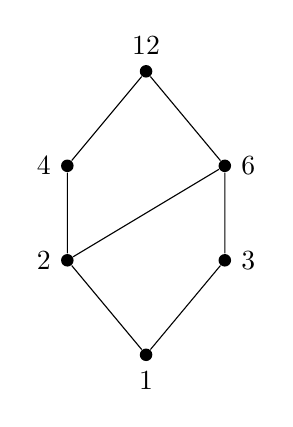
\begin{tikzpicture}[baseline=(current bounding box.center),scale=1.0]
\tikzset{pt/.style={circle,fill,inner sep=1.6pt}}
\node (1) at (0,0) [pt,label=below:$1$] {};
\node (2) at (-1,1.2) [pt,label=left:$2$] {};
\node (3) at (1,1.2) [pt,label=right:$3$] {};
\node (4) at (-1,2.4) [pt,label=left:$4$] {};
\node (6) at (1,2.4) [pt,label=right:$6$] {};
\node (12) at (0,3.6) [pt,label=above:$12$] {};
\draw (1)--(2) (1)--(3) (2)--(4) (2)--(6) (3)--(6) (4)--(12) (6)--(12);
\end{tikzpicture}
\]

\medskip
\textbf{Mô tả các phạm trù tương ứng.}
\begin{itemize}
  \item \emph{Phạm trù từ preorder $(\Omega,\mid)$:} đặt $\Ob(\mathbf{\Omega})=\Omega$ và
  \[
  \Hom_{\mathbf{\Omega}}(a,b)=
  \begin{cases}
  \{\ast\}, & a\mid b,\\
  \varnothing, & \text{ngược lại.}
  \end{cases}
  \]
  % Đây là \emph{phạm trù mảnh} (thin category). 
  
  Vì $a\mid -a$ và $-a\mid a$ nên 
  $a$ và $-a$ là \emph{đẳng cấu} trong $\mathbf{\Omega}$ (có mũi tên hai chiều).
  Do đó $\mathbf{\Omega}$ \emph{không} là poset–category.
  \item \emph{Phạm trù từ poset $(\Omega_+,\mid)$:} tương tự, đặt
  $\Ob(\mathbf{\Omega}_+)=\Omega_+$ và định nghĩa $\Hom$ như trên. 
  Lúc này nếu có mũi tên hai chiều thì tất yếu $a=b$, nên $\mathbf{\Omega}_+$ là 
  \emph{poset–category}.
  % (mảnh và phản đối xứng).
\end{itemize}

% \noindent
% \emph{Nhận xét.} Lấy \emph{bộ xương} (skeleton) của $\mathbf{\Omega}$ chính là 
% $\mathbf{\Omega}_+$: ta gom các cặp đẳng cấu $\{a,-a\}$ thành một đối tượng duy nhất.
\end{proof}


\begin{exercise}[10]
    Xét các kiểu cấu xạ trong từng phạm trù cụ thể (đơn cấu, toàn cấu, song cấu, đẳng cấu, tự đồng cấu, tự đẳng cấu, phép co rút, lát cắt).
\end{exercise}
\begin{proof}
    
\end{proof}

\begin{exercise}[11]
    Chứng minh mọi phép co rút đều là toàn cấu và mọi lát cắt đều là đơn cấu.
\end{exercise}
\begin{proof}
    \begin{proposition}[Mệnh đề 11]
Trong một phạm trù bất kỳ:
\begin{enumerate}
  \item Mọi \emph{phép co rút} (retraction) đều là \emph{toàn cấu} (epimorphism).
  \item Mọi \emph{lát cắt} (section) đều là \emph{đơn cấu} (monomorphism).
\end{enumerate}
\end{proposition}

\begin{proof}
Gọi $f:a\to b$ là một cấu xạ.

\smallskip
\noindent\textbf{(1) Co rút $\Rightarrow$ toàn cấu.}
Giả sử $f$ là \emph{co rút}, tức tồn tại $r:b\to a$ sao cho
\[
f\circ r = \Id_b.
\]
Lấy hai cấu xạ bất kỳ $g_1,g_2:b\to c$ và giả sử $g_1\circ f = g_2\circ f$.
Khi đó
\[
g_1
= g_1\circ \Id_b
= g_1\circ (f\circ r)
= (g_1\circ f)\circ r
= (g_2\circ f)\circ r
= g_2\circ (f\circ r)
= g_2\circ \Id_b
= g_2.
\]
Suy ra $g_1=g_2$, nên $f$ là \emph{epimorphism}.

\smallskip
\noindent\textbf{(2) Lát cắt $\Rightarrow$ đơn cấu.}
Giả sử $f$ là \emph{lát cắt}, tức tồn tại $s:b\to a$ sao cho
\[
s\circ f = \Id_a.
\]
Cho $h_1,h_2:x\to a$ và giả sử $f\circ h_1 = f\circ h_2$. Khi đó
\[
h_1
= \Id_a\circ h_1
= (s\circ f)\circ h_1
= s\circ (f\circ h_1)
= s\circ (f\circ h_2)
= (s\circ f)\circ h_2
= \Id_a\circ h_2
= h_2.
\]
Do đó $h_1=h_2$, tức $f$ là \emph{monomorphism}.
\end{proof}

\begin{remark}
Hai khẳng định trên là \emph{đối ngẫu} của nhau: thay \(\mathcal C\) bởi \(\mathcal C^{\mathrm{op}}\)
thì “co rút $\Rightarrow$ toàn cấu” chuyển thành “lát cắt $\Rightarrow$ đơn cấu”.
Chú ý: đảo chiều hàm kéo theo đổi vai \emph{epi} $\leftrightarrow$ \emph{mono}.
\end{remark}

\end{proof}

\begin{exercise}[12]
    Phải chăng mỗi toàn cấu là một phép co rút?

    Phải chăng mỗi đơn cấu là một lát cắt?
\end{exercise}
\begin{proof}
    \begin{proposition}
Không phải mọi toàn cấu đều là phép co rút, 
và không phải mọi đơn cấu đều là lát cắt.
\end{proposition}

\begin{proof}
\textbf{(1) Toàn cấu không nhất thiết là phép co rút.}

Xét phạm trù $\mathbf{Set}$.
Một \emph{toàn cấu} $f : A \to B$ là một ánh xạ \emph{toàn ánh},
tức là $f(A)=B$. 
Một \emph{phép co rút} yêu cầu tồn tại $r : B \to A$ sao cho
\[
f \circ r = 1_B.
\]
Nói cách khác, $r$ là một \emph{nghịch đảo phải} của $f$.

\smallskip
\textbf{Phản ví dụ:}
Xét hàm $f:\mathbb{N}\to\{0,1\}$ xác định bởi
\[
f(n) =
\begin{cases}
0, & \text{n chẵn},\\
1, & \text{n lẻ.}
\end{cases}
\]
Hàm $f$ là \emph{toàn ánh}, nên $f$ là toàn cấu trong $\mathbf{Set}$.
Tuy nhiên, không tồn tại hàm $r:\{0,1\}\to\mathbb{N}$ sao cho $f\circ r = 1_{\{0,1\}}$:
điều đó đòi hỏi $f(r(0))=0$ và $f(r(1))=1$, nhưng ta không thể định nghĩa duy nhất
$r(0),r(1)$ sao cho đẳng thức này đúng với mọi phần tử (nhiều lựa chọn khác nhau cho $r$).
Dù tồn tại lựa chọn có thể làm $f\circ r=1_B$ nếu dùng quy tắc chọn, 
song trong phạm trù $\mathbf{Set}$ điều này không \emph{bắt buộc}.

Vì vậy $f$ là toàn cấu nhưng \emph{không} là phép co rút.

\medskip
\textbf{(2) Đơn cấu không nhất thiết là lát cắt.}

Một \emph{đơn cấu} $f : A \to B$ trong $\mathbf{Set}$ là một ánh xạ \emph{đơn ánh}.
Một \emph{lát cắt} yêu cầu tồn tại $s : B \to A$ sao cho
\[
s \circ f = 1_A,
\]
tức $s$ là \emph{nghịch đảo trái} của $f$.

\smallskip
\textbf{Phản ví dụ:}
Xét phép chèn $f:\mathbb{N}\hookrightarrow\mathbb{Z}$, $f(n)=n$.

Rõ ràng $f$ là đơn ánh, nên $f$ là đơn cấu trong $\mathbf{Set}$.
Tuy nhiên, không tồn tại ánh xạ $s:\mathbb{Z}\to\mathbb{N}$ sao cho
$s\circ f = 1_{\mathbb{N}}$, vì với $z<0$, $s(z)$ không thể xác định sao cho thỏa mãn đẳng thức này.
Do đó $f$ không phải là lát cắt.

\medskip
\textbf{(3) Kết luận tổng quát:}
\begin{align*}
&\text{Nếu } f \text{ là phép co rút} \Rightarrow f \text{ là toàn cấu, nhưng không ngược lại;}\\[2pt]
&\text{Nếu } f \text{ là lát cắt} \Rightarrow f \text{ là đơn cấu, nhưng không ngược lại.}
\end{align*}
\end{proof}

\begin{remark}
Hai mệnh đề này là \emph{đối ngẫu} của nhau:
nếu ta xét phạm trù đối $\mathcal{C}^{\mathrm{op}}$, 
thì “toàn cấu” biến thành “đơn cấu” và “co rút” biến thành “lát cắt”.

\medskip
Sơ đồ logic giữa các khái niệm có thể tóm tắt như sau:
\[
\begin{tikzcd}[row sep=large, column sep=huge]
\text{lát cắt} \arrow[r,Rightarrow,"\text{nghịch đảo trái}"] & \text{đơn cấu}\\
\text{co rút} \arrow[r,Rightarrow,"\text{nghịch đảo phải}"] & \text{toàn cấu}
\end{tikzcd}
\]
Các mũi tên ở đây \emph{không khả nghịch} nói chung.
\end{remark}

\end{proof}

\begin{exercise}[13]
    Cho $f$ là một cấu xạ trong một phạm trù $\mathcal{C}$. Ba khẳng định sau là một tương đương với nhau
    \begin{itemize}
        \item $f$ là một đơn cấu và là một phép co rút.

        \item $f$ là một toàn cấu và là một lát cắt.

        \item $f$ là một đẳng cấu.
    \end{itemize}
\end{exercise}

\begin{proof}
\textbf{(3) $\Rightarrow$ (1) và (2).}

Nếu $f$ là đẳng cấu thì tồn tại nghịch đảo $f^{-1}:b\to a$ với
$f\circ f^{-1}=1_b$ và $f^{-1}\circ f=1_a$. Do đó $f$ vừa là co rút (với $r=f^{-1}$),
vừa là lát cắt (với $s=f^{-1}$), và vì đẳng cấu luôn vừa đơn cấu vừa toàn cấu,
nên (1) và (2) đều đúng.

\medskip
\textbf{(1) $\Rightarrow$ (3).}

Giả sử $f$ là đơn cấu và tồn tại $r:b\to a$ sao cho $f\circ r=1_b$.
Xét hai cấu xạ $r\circ f,\,1_a:a\to a$. Ta có
\[
f\circ(r\circ f)=(f\circ r)\circ f=1_b\circ f=f
\qquad\text{và}\qquad
f\circ 1_a=f.
\]
Vì $f$ là đơn cấu nên suy ra $r\circ f=1_a$. Như vậy $r$ là nghịch đảo hai phía của $f$,
nên $f$ là đẳng cấu.

\medskip
\textbf{(2) $\Rightarrow$ (3).}

Giả sử $f$ là toàn cấu và tồn tại $s:b\to a$ sao cho $s\circ f=1_a$.
Xét hai cấu xạ $f\circ s,\,1_b:b\to b$. Ta có
\[
(f\circ s)\circ f=f\circ(s\circ f)=f\circ 1_a=f
\qquad\text{và}\qquad
1_b\circ f=f.
\]
Vì $f$ là toàn cấu nên suy ra $f\circ s=1_b$. Khi đó $s$ là nghịch đảo hai phía của $f$,
nên $f$ là đẳng cấu.

% \medskip
% Kết luận: (1)$\Leftrightarrow$(3)$\Leftrightarrow$(2).

% \begin{remark}
% Hai hướng (1)$\Rightarrow$(3) và (2)$\Rightarrow$(3) là \emph{đối ngẫu} của nhau:
% đổi $\mathcal C$ bởi $\mathcal C^{\mathrm{op}}$ sẽ hoán đổi ``đơn cấu–lát cắt''
% với ``toàn cấu–co rút''. 
% \end{remark}

\end{proof}

\begin{exercise}[14]
    Giải thích mối liên hệ giữa đẳng cấu và song cấu.
\end{exercise}
    \begin{proposition}
Mọi đẳng cấu đều là song cấu (tức vừa đơn cấu vừa toàn cấu).
\end{proposition}

\begin{proof}
Giả sử $f:A\to B$ là một \emph{đẳng cấu}, nên tồn tại nghịch đảo hai phía
$g:B\to A$ với $g\circ f=1_A$ và $f\circ g=1_B$.

\emph{(Đơn cấu).} Lấy $u,v:X\to A$ và giả sử $f\circ u=f\circ v$. Khi đó
\[
u=1_A\circ u=(g\circ f)\circ u=g\circ(f\circ u)
      =g\circ(f\circ v)=(g\circ f)\circ v=1_A\circ v=v.
\]
Suy ra $f$ là đơn cấu.

\emph{(Toàn cấu).} Lấy $p,q:B\to Y$ và giả sử $p\circ f=q\circ f$. Khi đó
\[
p=p\circ 1_B=p\circ(f\circ g)=(p\circ f)\circ g
       =(q\circ f)\circ g=q\circ(f\circ g)=q\circ 1_B=q.
\]
Suy ra $f$ là toàn cấu. Vậy $f$ là \emph{song cấu}.

\begin{remark}[Mối liên hệ giữa các kiểu cấu xạ]
Các khái niệm cơ bản trong phạm trù học có mối quan hệ như sau:

\begin{itemize}
  \item Mọi \textbf{đẳng cấu} đều là \textbf{song cấu} (tức vừa đơn cấu vừa toàn cấu).
  \item Mọi \textbf{lát cắt} là \textbf{đơn cấu}.
  \item Mọi \textbf{phép co rút} là \textbf{toàn cấu}.
  \item Ngược lại, các chiều đảo thường không đúng:
  \[
  \text{đơn cấu } \not\Rightarrow \text{ lát cắt}, \qquad
  \text{toàn cấu } \not\Rightarrow \text{ co rút}, \qquad
  \text{song cấu } \not\Rightarrow \text{ đẳng cấu}.
  \]
  \item Tuy nhiên, ta có các tương đương mạnh hơn:
  \[
  \boxed{
  \begin{aligned}
  f \text{ là đơn cấu và co rút} &\iff f \text{ là đẳng cấu},\\[4pt]
  f \text{ là toàn cấu và lát cắt} &\iff f \text{ là đẳng cấu}.
  \end{aligned}}
  \]
\end{itemize}
\end{remark}

\end{proof}

\begin{exercise}[20]
Xác định các kiểu cấu xạ: đơn cấu, toàn cấu, song cấu, đẳng cấu, phép co rút, lát cắt 
trong phạm trù $\mathbf{Set}$.
\end{exercise}

\begin{proof}
Trong phạm trù $\mathbf{Set}$, các vật là các tập hợp, và các cấu xạ là các \emph{hàm} giữa các tập hợp.  
Ta mô tả từng loại cấu xạ như sau:

\medskip
\noindent
\textbf{1. Đơn cấu (Monomorphism).}  
Một cấu xạ $f:A\to B$ là \emph{đơn cấu} nếu
\[
f\circ g_1 = f\circ g_2 \implies g_1 = g_2
\]
với mọi $g_1,g_2:X\to A$.

Trong $\mathbf{Set}$, điều này tương đương với $f$ là \emph{đơn ánh (injective)}.  
Thật vậy, nếu $f$ không đơn ánh thì tồn tại $x_1\ne x_2$ sao cho $f(x_1)=f(x_2)$; 
lấy $X=\{*\}$ và đặt $g_i(*)=x_i$ thì $f\circ g_1=f\circ g_2$ nhưng $g_1\ne g_2$.  
Ngược lại, nếu $f$ đơn ánh thì $f\circ g_1=f\circ g_2$ kéo theo $g_1=g_2$ từng phần tử.

\[
\boxed{f \text{ đơn cấu } \iff f \text{ đơn ánh.}}
\]

\medskip
\noindent
\textbf{2. Toàn cấu (Epimorphism).}  
Một cấu xạ $f:A\to B$ là \emph{toàn cấu} nếu
\[
g_1\circ f = g_2\circ f \implies g_1=g_2
\]
với mọi $g_1,g_2:B\to C$.

Trong $\mathbf{Set}$, điều này tương đương với $f$ là \emph{toàn ánh (surjective)}.  
Nếu $f$ không toàn ánh, chọn $b_0\in B\setminus f(A)$, và định nghĩa $g_1,g_2:B\to\{0,1\}$ khác nhau tại $b_0$ 
(nhưng đồng nhất trên $f(A)$), ta được $g_1\circ f=g_2\circ f$ nhưng $g_1\ne g_2$.  
Ngược lại, nếu $f$ toàn ánh thì hai hàm $g_1,g_2$ trùng trên $f(A)=B$, nên $g_1=g_2$.

\[
\boxed{f \text{ toàn cấu } \iff f \text{ toàn ánh.}}
\]

\medskip
\noindent
\textbf{3. Song cấu (Bimorphism).}  
$f$ là \emph{song cấu} nếu vừa đơn cấu vừa toàn cấu.  
Trong $\mathbf{Set}$, điều này nghĩa là $f$ vừa \emph{đơn ánh} vừa \emph{toàn ánh}, tức là \emph{song ánh}.

\[
\boxed{f \text{ song cấu } \iff f \text{ song ánh.}}
\]

\medskip
\noindent
\textbf{4. Đẳng cấu (Isomorphism).}  
$f:A\to B$ là \emph{đẳng cấu} nếu tồn tại $g:B\to A$ sao cho
\[
f\circ g = 1_B, \quad g\circ f = 1_A.
\]
Trong $\mathbf{Set}$, điều này tương đương với $f$ có \emph{nghịch đảo hai phía}, 
tức là $f$ là \emph{song ánh} (vì hàm song ánh có nghịch đảo đúng bằng hàm ngược).

\[
\boxed{f \text{ đẳng cấu } \iff f \text{ song ánh.}}
\]
Do đó trong $\mathbf{Set}$, “song cấu” và “đẳng cấu” trùng nhau.

\medskip
\noindent
\textbf{5. Phép co rút (Retraction).}  
$f:A\to B$ là \emph{phép co rút} nếu tồn tại $r:B\to A$ sao cho
\[
f\circ r = 1_B.
\]
Điều này có nghĩa là $r$ là một \emph{phép chọn} ngược cho $f$, 
tức là $f$ \emph{phủ toàn bộ $B$} (mỗi phần tử $b\in B$ có ít nhất một $a\in A$ với $f(a)=b$).

\[
\boxed{f \text{ là phép co rút } \iff f \text{ là toàn ánh.}}
\]

\medskip
\noindent
\textbf{6. Lát cắt (Section).}  
$f:A\to B$ là \emph{lát cắt} nếu tồn tại $s:B\to A$ sao cho
\[
s\circ f = 1_A.
\]
Nghĩa là $f$ có nghịch đảo trái, tương đương với việc $f$ \emph{đơn ánh} trong $\mathbf{Set}$.

\[
\boxed{f \text{ là lát cắt } \iff f \text{ là đơn ánh.}}
\]

\medskip
\noindent
\textbf{Kết luận tổng hợp:}
\[
\begin{array}{lcl}
\text{Đơn cấu} &\Longleftrightarrow& \text{đơn ánh},\\[3pt]
\text{Toàn cấu} &\Longleftrightarrow& \text{toàn ánh},\\[3pt]
\text{Song cấu} &\Longleftrightarrow& \text{song ánh},\\[3pt]
\text{Đẳng cấu} &\Longleftrightarrow& \text{song ánh},\\[3pt]
\text{Phép co rút} &\Longleftrightarrow& \text{toàn ánh},\\[3pt]
\text{Lát cắt} &\Longleftrightarrow& \text{đơn ánh.}
\end{array}
\]
Vì vậy phạm trù $\mathbf{Set}$ là một \emph{phạm trù cân bằng}:
\[
\text{Đơn cấu + Toàn cấu } \iff \text{Đẳng cấu.}
\]
\end{proof}

\begin{exercise}[21]
Xác định các kiểu cấu xạ: đơn cấu, toàn cấu, song cấu, đẳng cấu, 
phép co rút, lát cắt trong phạm trù $\mathbf{Vect}_K$.
\end{exercise}

\begin{proof}
Trong phạm trù $\mathbf{Vect}_K$, các vật là các không gian vector trên trường $K$, 
và các cấu xạ là các ánh xạ tuyến tính giữa chúng.  

\medskip
\noindent
\textbf{1. Đơn cấu (Monomorphism).}  
Một ánh xạ tuyến tính $f:V\to W$ là \emph{đơn cấu} nếu
\[
f\circ g_1 = f\circ g_2 \implies g_1 = g_2
\]
với mọi ánh xạ tuyến tính $g_1,g_2:U\to V$.  
Trong $\mathbf{Vect}_K$, điều này tương đương với $f$ là \emph{đơn ánh (injective)}.

Thật vậy, nếu $f$ không đơn ánh thì tồn tại $v_1\ne v_2$ sao cho $f(v_1)=f(v_2)$, 
suy ra tồn tại $g_1,g_2$ từ $K$ vào $V$ với $g_i(1)=v_i$ thỏa $f\circ g_1=f\circ g_2$ nhưng $g_1\ne g_2$.  
Ngược lại, nếu $f$ đơn ánh thì $f\circ g_1=f\circ g_2$ kéo theo $g_1=g_2$ từng phần tử.

\[
\boxed{f \text{ đơn cấu } \iff f \text{ đơn ánh.}}
\]

\medskip
\noindent
\textbf{2. Toàn cấu (Epimorphism).}  
Một ánh xạ tuyến tính $f:V\to W$ là \emph{toàn cấu} nếu
\[
g_1\circ f = g_2\circ f \implies g_1=g_2
\]
với mọi ánh xạ tuyến tính $g_1,g_2:W\to Z$.  
Điều này tương đương với $f$ là \emph{toàn ánh (surjective)}.

Nếu $f$ không toàn ánh, chọn $w_0\notin \operatorname{Im}(f)$, 
và định nghĩa $g_1,g_2:W\to K$ sao cho $g_1(w_0)\ne g_2(w_0)$ nhưng $g_1,g_2$ trùng nhau trên $\operatorname{Im}(f)$; 
khi đó $g_1\circ f=g_2\circ f$ nhưng $g_1\ne g_2$.  
Ngược lại, nếu $f$ toàn ánh thì $\operatorname{Im}(f)=W$, nên $g_1\circ f=g_2\circ f$ kéo theo $g_1=g_2$.

\[
\boxed{f \text{ toàn cấu } \iff f \text{ toàn ánh.}}
\]

\medskip
\noindent
\textbf{3. Song cấu (Bimorphism).}  
$f$ là \emph{song cấu} nếu vừa đơn cấu vừa toàn cấu.  
Khi đó $f$ vừa đơn ánh vừa toàn ánh, nghĩa là $f$ là \emph{đẳng cấu tuyến tính (isomorphism)}.

\[
\boxed{f \text{ song cấu } \iff f \text{ đẳng cấu.}}
\]

\medskip
\noindent
\textbf{4. Đẳng cấu (Isomorphism).}  
Một ánh xạ tuyến tính $f:V\to W$ là \emph{đẳng cấu} nếu tồn tại $g:W\to V$ sao cho
\[
f\circ g = 1_W, \quad g\circ f = 1_V.
\]
Trong $\mathbf{Vect}_K$, điều này đúng khi và chỉ khi $f$ là \emph{song ánh}.  
Đồng thời, $f$ khi đó là \emph{nghịch đảo tuyến tính}, nên:
\[
\boxed{f \text{ đẳng cấu } \iff f \text{ song ánh (đẳng cấu tuyến tính)}.}
\]

\medskip
\noindent
\textbf{5. Phép co rút (Retraction).}  
$f:V\to W$ là \emph{phép co rút} nếu tồn tại ánh xạ tuyến tính $r:W\to V$ sao cho
\[
f\circ r = 1_W.
\]
Tức là $r$ là \emph{phép nghịch đảo phải} của $f$.  
Điều này xảy ra khi và chỉ khi $f$ là \emph{toàn ánh}.  
Thật vậy, từ $f\circ r = 1_W$ suy ra với mọi $w\in W$, tồn tại $v=r(w)$ sao cho $f(v)=w$.

\[
\boxed{f \text{ là phép co rút } \iff f \text{ là toàn ánh.}}
\]

\medskip
\noindent
\textbf{6. Lát cắt (Section).}  
$f:V\to W$ là \emph{lát cắt} nếu tồn tại ánh xạ tuyến tính $s:W\to V$ sao cho
\[
s\circ f = 1_V.
\]
Tức là $f$ có nghịch đảo trái, nên $f$ \emph{đơn ánh}.  
Ngược lại, nếu $f$ đơn ánh, có thể chọn không gian con bù $U$ của $\operatorname{Im}(f)$ sao cho $W=f(V)\oplus U$, 
và định nghĩa $s$ là nghịch đảo của $f$ trên $f(V)$ và bằng $0$ trên $U$. Khi đó $s$ tuyến tính và $s\circ f = 1_V$.

\[
\boxed{f \text{ là lát cắt } \iff f \text{ là đơn ánh.}}
\]

\medskip
\noindent
\textbf{Kết luận tổng hợp:}
\[
\begin{array}{lcl}
\text{Đơn cấu} &\Longleftrightarrow& \text{đơn ánh},\\[3pt]
\text{Toàn cấu} &\Longleftrightarrow& \text{toàn ánh},\\[3pt]
\text{Song cấu} &\Longleftrightarrow& \text{đẳng cấu},\\[3pt]
\text{Đẳng cấu} &\Longleftrightarrow& \text{song ánh},\\[3pt]
\text{Phép co rút} &\Longleftrightarrow& \text{toàn ánh},\\[3pt]
\text{Lát cắt} &\Longleftrightarrow& \text{đơn ánh.}
\end{array}
\]

\noindent
Vì vậy, phạm trù $\mathbf{Vect}_K$ là một \emph{phạm trù cân bằng}:
\[
\text{Đơn cấu + Toàn cấu } \iff \text{Đẳng cấu.}
\]
\end{proof}

\begin{exercise}[22]
Xác định các kiểu cấu xạ: đơn cấu, toàn cấu, song cấu, đẳng cấu, 
phép co rút, lát cắt trong phạm trù $\mathbf{Grp}$.
\end{exercise}

\begin{proof}
Trong phạm trù $\mathbf{Grp}$, các vật là các nhóm, 
và các cấu xạ là các \emph{đồng cấu nhóm} (group homomorphisms).  
Ta xác định từng loại như sau:

\medskip
\noindent
\textbf{1. Đơn cấu (Monomorphism).}  
Một đồng cấu nhóm $f:G\to H$ là \emph{đơn cấu} nếu
\[
f\circ g_1 = f\circ g_2 \implies g_1 = g_2
\]
với mọi đồng cấu nhóm $g_1,g_2:K\to G$.  

Điều này tương đương với $f$ là \emph{đơn ánh}.  
Thật vậy:
\begin{itemize}
  \item Nếu $f$ không đơn ánh, tồn tại $x\ne y\in G$ với $f(x)=f(y)$, 
        xét $K=\mathbb{Z}$ và hai đồng cấu $g_1,g_2$ cho bởi $g_1(1)=x$, $g_2(1)=y$, 
        khi đó $f\circ g_1 = f\circ g_2$ nhưng $g_1\ne g_2$.
  \item Ngược lại, nếu $f$ đơn ánh thì $f\circ g_1 = f\circ g_2$ 
        kéo theo $g_1=g_2$ vì $f$ không đồng nhất hai phần tử khác nhau.
\end{itemize}
Do đó:
\[
\boxed{f \text{ đơn cấu } \iff f \text{ đơn ánh.}}
\]

\medskip
\noindent
\textbf{2. Toàn cấu (Epimorphism).}  
Một đồng cấu $f:G\to H$ là \emph{toàn cấu} nếu
\[
g_1\circ f = g_2\circ f \implies g_1 = g_2
\]
với mọi $g_1,g_2:H\to K$.  

Trong $\mathbf{Grp}$, điều này tương đương với $f$ là \emph{toàn ánh}.  
Thật vậy:
\begin{itemize}
  \item Nếu $f$ toàn ánh thì rõ ràng $g_1\circ f=g_2\circ f$ kéo theo $g_1=g_2$.
  \item Nếu $f$ không toàn ánh, tồn tại $h_0\in H\setminus f(G)$.  
        Xét $K=H/\langle h_0 \rangle$ và định nghĩa hai đồng cấu $g_1,g_2:H\to K$
        khác nhau tại $h_0$ nhưng trùng nhau trên $f(G)$; khi đó $g_1\circ f=g_2\circ f$.
\end{itemize}
\[
\boxed{f \text{ toàn cấu } \iff f \text{ toàn ánh.}}
\]

\medskip
\noindent
\textbf{3. Song cấu (Bimorphism).}  
$f$ là \emph{song cấu} nếu vừa đơn cấu vừa toàn cấu, tức vừa đơn ánh vừa toàn ánh.  
Như vậy:
\[
\boxed{f \text{ song cấu } \iff f \text{ là đồng cấu song ánh.}}
\]
Song ánh đồng cấu nhóm chính là đẳng cấu, nên trong $\mathbf{Grp}$: song cấu = đẳng cấu.

\medskip
\noindent
\textbf{4. Đẳng cấu (Isomorphism).}  
$f:G\to H$ là \emph{đẳng cấu} nếu tồn tại đồng cấu $g:H\to G$ sao cho
\[
f\circ g = 1_H, \qquad g\circ f = 1_G.
\]
Khi đó $f$ là song ánh và $g=f^{-1}$ là nghịch đảo nhóm học.

\[
\boxed{f \text{ đẳng cấu } \iff f \text{ song ánh (đồng cấu nghịch đảo).}}
\]

\medskip
\noindent
\textbf{5. Phép co rút (Retraction).}  
$f:G\to H$ là \emph{phép co rút} nếu tồn tại đồng cấu $r:H\to G$ sao cho
\[
f\circ r = 1_H.
\]
Điều này có nghĩa $r$ là \emph{nghịch đảo phải} của $f$.  
Vì vậy $f$ phải là \emph{toàn ánh}, và ta có $H \cong f(G)$ là một ảnh đồng cấu của $G$.  
Nếu tồn tại $r$ như vậy, ta nói rằng $H$ là \emph{nhóm thương trực tiếp} của $G$.

\[
\boxed{f \text{ là phép co rút } \Rightarrow f \text{ là toàn ánh.}}
\]

\medskip
\noindent
\textbf{6. Lát cắt (Section).}  
$f:G\to H$ là \emph{lát cắt} nếu tồn tại đồng cấu $s:H\to G$ sao cho
\[
s\circ f = 1_G.
\]
Điều này nghĩa là $f$ có nghịch đảo trái, nên $f$ là \emph{đơn ánh}.  
Ngược lại, không phải mọi đơn ánh đều là lát cắt, 
vì cần tồn tại phép “tách” nhóm đích thành tích trực tiếp:
\[
H \cong f(G) \times K \quad \text{với $K$ là một nhóm con bổ sung.}
\]
Ví dụ: bao hàm $\iota:\mathbb{Z}\hookrightarrow\mathbb{Q}$ là đơn ánh nhưng không có lát cắt 
(vì không có đồng cấu $\mathbb{Q}\to\mathbb{Z}$ thoả $\iota\circ s = 1_{\mathbb{Z}}$).

\[
\boxed{f \text{ là lát cắt } \Rightarrow f \text{ là đơn ánh, nhưng không ngược lại.}}
\]

\medskip
\noindent
\textbf{Kết luận tổng hợp:}
\[
\begin{array}{lcl}
\text{Đơn cấu} &\Longleftrightarrow& \text{đồng cấu đơn ánh},\\[3pt]
\text{Toàn cấu} &\Longleftrightarrow& \text{đồng cấu toàn ánh},\\[3pt]
\text{Song cấu} &\Longleftrightarrow& \text{đồng cấu song ánh},\\[3pt]
\text{Đẳng cấu} &\Longleftrightarrow& \text{đồng cấu nghịch đảo},\\[3pt]
\text{Phép co rút} &\Longrightarrow& \text{toàn ánh (có nghịch đảo phải)},\\[3pt]
\text{Lát cắt} &\Longrightarrow& \text{đơn ánh (có nghịch đảo trái).}
\end{array}
\]
Ngoài ra, $\mathbf{Grp}$ là một \emph{phạm trù cân bằng}:
\[
\text{Đơn cấu + Toàn cấu } \iff \text{Đẳng cấu.}
\]
\end{proof}

\begin{exercise}[23]
Xác định các kiểu cấu xạ: đơn cấu, toàn cấu, song cấu, đẳng cấu, 
phép co rút, lát cắt trong phạm trù $\mathbf{Top}$.
\end{exercise}

\begin{proof}
Trong phạm trù $\mathbf{Top}$, các vật là các không gian tôpô, 
và các cấu xạ là các \emph{ánh xạ liên tục}.  
Ta mô tả từng loại như sau:

\medskip
\noindent
\textbf{1. Đơn cấu (Monomorphism).}  
Một ánh xạ liên tục $f:X\to Y$ là \emph{đơn cấu} nếu
\[
f\circ g_1 = f\circ g_2 \implies g_1 = g_2
\]
với mọi ánh xạ liên tục $g_1,g_2:Z\to X$.

Trong $\mathbf{Top}$, điều này tương đương với $f$ là \emph{hàm đơn ánh}.  
Thật vậy:
\begin{itemize}
  \item Nếu $f$ không đơn ánh, tồn tại $x_1\ne x_2$ sao cho $f(x_1)=f(x_2)$, 
  khi đó lấy $Z$ là một điểm và định nghĩa hai ánh xạ hằng $g_i(*)=x_i$, 
  ta có $f\circ g_1=f\circ g_2$ nhưng $g_1\ne g_2$.
  \item Ngược lại, nếu $f$ đơn ánh, thì $f\circ g_1=f\circ g_2$ kéo theo $g_1=g_2$ từng điểm.
\end{itemize}

\[
\boxed{f \text{ đơn cấu } \iff f \text{ đơn ánh.}}
\]

Tuy nhiên, lưu ý rằng \emph{không cần} $f$ là nhúng tôpô (embedding); chỉ cần là hàm đơn ánh liên tục.

\medskip
\noindent
\textbf{2. Toàn cấu (Epimorphism).}  
Một ánh xạ liên tục $f:X\to Y$ là \emph{toàn cấu} nếu
\[
g_1\circ f = g_2\circ f \implies g_1=g_2
\]
với mọi ánh xạ liên tục $g_1,g_2:Y\to Z$.  

Khi đó, $f$ là \emph{toàn cấu} nếu ảnh $f(X)$ \emph{mật} trong $Y$.  
Thật vậy:
\begin{itemize}
  \item Nếu $f(X)$ là \emph{mật} trong $Y$, hai ánh xạ $g_1,g_2$ liên tục và trùng nhau trên $f(X)$ thì phải trùng nhau trên toàn bộ $Y$.
  \item Nếu $f(X)$ không mật, tồn tại một tập mở $U\subseteq Y$ với $U\cap f(X)=\varnothing$; ta có thể chọn hai ánh xạ $g_1,g_2$ khác nhau trên $U$ mà vẫn trùng nhau trên $f(X)$, nên $f$ không là toàn cấu.
\end{itemize}

\[
\boxed{f \text{ toàn cấu } \iff \overline{f(X)} = Y.}
\]

Như vậy, mọi ánh xạ toàn ánh là toàn cấu, nhưng tồn tại toàn cấu không toàn ánh 
(như bao gồm $\mathbb{Q}\hookrightarrow\mathbb{R}$).

\medskip
\noindent
\textbf{3. Song cấu (Bimorphism).}  
$f$ là \emph{song cấu} nếu vừa đơn cấu vừa toàn cấu.  
Điều này nghĩa là $f$ vừa đơn ánh, vừa có ảnh mật trong $Y$.  
Ví dụ: bao gồm $\mathbb{Q}\hookrightarrow\mathbb{R}$ là song cấu nhưng không đẳng cấu.

\[
\boxed{f \text{ song cấu } \iff f \text{ đơn ánh và } \overline{f(X)} = Y.}
\]

\medskip
\noindent
\textbf{4. Đẳng cấu (Isomorphism).}  
$f:X\to Y$ là \emph{đẳng cấu} nếu tồn tại $g:Y\to X$ liên tục sao cho
\[
f\circ g = 1_Y,\qquad g\circ f = 1_X.
\]
Điều này có nghĩa là $f$ là \emph{song ánh} và cả $f, f^{-1}$ đều liên tục, 
tức là $f$ là \emph{homeomorphism (phép đồng phôi tôpô)}.

\[
\boxed{f \text{ đẳng cấu } \iff f \text{ là đồng phôi tôpô.}}
\]

\medskip
\noindent
\textbf{5. Phép co rút (Retraction).}  
$f:X\to Y$ là \emph{phép co rút} nếu tồn tại $r:Y\to X$ liên tục sao cho
\[
f\circ r = 1_Y.
\]
Khi đó $Y$ được gọi là \emph{ảnh co rút} (retract) của $X$.  
Điều này có nghĩa rằng $Y$ là một không gian con của $X$ 
và phép bao gồm $i:Y\hookrightarrow X$ thỏa $f\circ i = 1_Y$.  
Ví dụ: hình tròn $S^1$ là một retract của đĩa đóng $\mathbb{D}^2$ 
qua phép chiếu $r(x) = \frac{x}{\|x\|}$.

\[
\boxed{f \text{ là phép co rút } \iff \exists\, r:Y\to X \text{ với } f\circ r=1_Y.}
\]

\medskip
\noindent
\textbf{6. Lát cắt (Section).}  
$f:X\to Y$ là \emph{lát cắt} nếu tồn tại $s:Y\to X$ liên tục sao cho
\[
s\circ f = 1_X.
\]
Tức là $f$ có \emph{nghịch đảo trái}.  
Điều này tương đương với việc $f$ là phép bao gồm (inclusion) của một không gian con $X\subseteq Y$, 
còn $s$ là phép chiếu (retraction) lên $X$.

\[
\boxed{f \text{ là lát cắt } \iff f \text{ là phép bao gồm có phép co rút.}}
\]

\medskip
\noindent
\textbf{Kết luận tổng hợp:}
\[
\begin{array}{lcl}
\text{Đơn cấu} &\Longleftrightarrow& \text{liên tục và đơn ánh},\\[3pt]
\text{Toàn cấu} &\Longleftrightarrow& \text{ảnh mật: } \overline{f(X)}=Y,\\[3pt]
\text{Song cấu} &\Longleftrightarrow& \text{đơn ánh, ảnh mật},\\[3pt]
\text{Đẳng cấu} &\Longleftrightarrow& \text{đồng phôi (homeomorphism)},\\[3pt]
\text{Phép co rút} &\Longleftrightarrow& \text{có nghịch đảo phải (retraction)},\\[3pt]
\text{Lát cắt} &\Longleftrightarrow& \text{có nghịch đảo trái (section).}
\end{array}
\]
Tuy nhiên, $\mathbf{Top}$ \emph{không phải là phạm trù cân bằng}, 
vì có song cấu không phải là đẳng cấu (ví dụ $\mathbb{Q}\hookrightarrow\mathbb{R}$).
\end{proof}

\begin{exercise}[24]
Xác định các kiểu cấu xạ: đơn cấu, toàn cấu, song cấu, đẳng cấu, 
phép co rút, lát cắt trong phạm trù $\mathbf{Mon}$.
\end{exercise}

\begin{proof}
Trong phạm trù $\mathbf{Mon}$, các vật là các vị nhóm (monoid), 
và các cấu xạ là các \emph{đồng cấu vị nhóm} 
$f:(M,\cdot,1_M)\to (N,\ast,1_N)$ thoả
\[
f(x\cdot y)=f(x)\ast f(y), \qquad f(1_M)=1_N.
\]
Ta sẽ phân tích từng loại cấu xạ:

\medskip
\noindent
\textbf{1. Đơn cấu (Monomorphism).}  
Một đồng cấu vị nhóm $f:M\to N$ là \emph{đơn cấu} nếu
\[
f\circ g_1 = f\circ g_2 \implies g_1 = g_2
\]
với mọi đồng cấu vị nhóm $g_1,g_2:K\to M$.  

Trong $\mathbf{Mon}$, điều này tương đương với $f$ là \emph{đơn ánh}.  
Lý do tương tự như trong $\mathbf{Grp}$:
\begin{itemize}
  \item Nếu $f$ không đơn ánh, tồn tại $x\ne y$ trong $M$ với $f(x)=f(y)$.  
        Lấy $K$ là vị nhóm tự do sinh bởi một phần tử $a$ (tức $K=\mathbb{N}$ với phép cộng), 
        định nghĩa $g_1(a)=x$, $g_2(a)=y$, ta có $f\circ g_1=f\circ g_2$ nhưng $g_1\ne g_2$.
  \item Ngược lại, nếu $f$ đơn ánh, thì $f\circ g_1=f\circ g_2$ kéo theo $g_1=g_2$.
\end{itemize}

\[
\boxed{f \text{ đơn cấu } \iff f \text{ đơn ánh.}}
\]

\medskip
\noindent
\textbf{2. Toàn cấu (Epimorphism).}  
Một đồng cấu vị nhóm $f:M\to N$ là \emph{toàn cấu} nếu
\[
g_1\circ f = g_2\circ f \implies g_1=g_2
\]
với mọi $g_1,g_2:N\to P$ đồng cấu vị nhóm.

Khác với $\mathbf{Grp}$, trong $\mathbf{Mon}$, không phải mọi toàn ánh đều là toàn cấu, 
và cũng có toàn cấu không toàn ánh.  

\begin{itemize}
  \item Nếu $f$ toàn ánh, rõ ràng là toàn cấu.
  \item Nhưng có ví dụ ngược: bao hàm $f:\mathbb{N}\hookrightarrow\mathbb{Z}$ 
        là \emph{toàn cấu} trong $\mathbf{Mon}$ (vì mọi đồng cấu $g_1,g_2:\mathbb{Z}\to P$ 
        bị xác định duy nhất bởi giá trị tại $1$), nhưng không toàn ánh.
\end{itemize}

\[
\boxed{f \text{ toàn cấu } \not\Rightarrow f \text{ toàn ánh.}}
\]
Tuy nhiên, mọi toàn ánh đều là toàn cấu.

\medskip
\noindent
\textbf{3. Song cấu (Bimorphism).}  
$f$ là \emph{song cấu} nếu vừa đơn cấu vừa toàn cấu.  
Khi đó $f$ vừa đơn ánh vừa toàn cấu.  
Nhưng trong $\mathbf{Mon}$, một song cấu không nhất thiết là đẳng cấu.

Ví dụ:  
Bao hàm $f:\mathbb{N}\hookrightarrow\mathbb{Z}$ là đơn ánh (nên đơn cấu) và cũng là toàn cấu (như trên), 
nhưng không có nghịch đảo, nên không phải đẳng cấu.

\[
 \boxed{f \text{ song cấu } \not\Rightarrow f \text{ đẳng cấu.}}
\]

\medskip
\noindent
\textbf{4. Đẳng cấu (Isomorphism).}  
Một đồng cấu $f:M\to N$ là \emph{đẳng cấu} nếu tồn tại $g:N\to M$ đồng cấu sao cho
\[
f\circ g = 1_N, \qquad g\circ f = 1_M.
\]
Khi đó $f$ là song ánh, và nghịch đảo $f^{-1}$ cũng là đồng cấu vị nhóm.

\[
\boxed{f \text{ đẳng cấu } \iff f \text{ song ánh và } f^{-1} \text{ là đồng cấu vị nhóm.}}
\]

\medskip
\noindent
\textbf{5. Phép co rút (Retraction).}  
$f:M\to N$ là \emph{phép co rút} nếu tồn tại đồng cấu $r:N\to M$ sao cho
\[
f\circ r = 1_N.
\]
Điều này nghĩa là $r$ là \emph{nghịch đảo phải} của $f$, 
nên $f$ là \emph{toàn ánh}.  
Hơn nữa, $N$ có thể được xem là một \emph{ảnh đồng cấu} của $M$ (một “retract” của $M$).

\[
\boxed{f \text{ là phép co rút } \Rightarrow f \text{ toàn ánh.}}
\]

\medskip
\noindent
\textbf{6. Lát cắt (Section).}  
$f:M\to N$ là \emph{lát cắt} nếu tồn tại $s:N\to M$ sao cho
\[
s\circ f = 1_M.
\]
Khi đó $f$ có nghịch đảo trái, nên $f$ \emph{đơn ánh}.  
Tuy nhiên, không phải mọi đơn ánh đều có lát cắt.

Ví dụ: bao hàm $f:\mathbb{N}\hookrightarrow\mathbb{Z}$ là đơn ánh 
nhưng không có đồng cấu $s:\mathbb{Z}\to\mathbb{N}$ 
(vì $s(-1)$ không thể xác định thỏa $s(x+y)=s(x)+s(y)$).

\[
\boxed{f \text{ là lát cắt } \Rightarrow f \text{ đơn ánh, nhưng không ngược lại.}}
\]

\medskip
\noindent
\textbf{Kết luận tổng hợp:}
\[
\begin{array}{lcl}
\text{Đơn cấu} &\Longleftrightarrow& \text{đồng cấu đơn ánh},\\[3pt]
\text{Toàn cấu} &\Longrightarrow& \text{toàn ánh (nhưng không ngược lại)},\\[3pt]
\text{Song cấu} &\Longleftrightarrow& \text{đơn ánh và toàn cấu (không nhất thiết đẳng cấu)},\\[3pt]
\text{Đẳng cấu} &\Longleftrightarrow& \text{song ánh và nghịch đảo là đồng cấu},\\[3pt]
\text{Phép co rút} &\Longrightarrow& \text{toàn ánh},\\[3pt]
\text{Lát cắt} &\Longrightarrow& \text{đơn ánh.}
\end{array}
\]
Phạm trù $\mathbf{Mon}$ \emph{không cân bằng}, 
vì tồn tại song cấu không phải đẳng cấu 
(ví dụ $\mathbb{N}\hookrightarrow\mathbb{Z}$).
\end{proof}


\begin{exercise}[25]
\leavevmode
\begin{enumerate}
    \item Phải chăng mỗi toàn cấu là một phép co rút?
    \item Phải chăng mỗi đơn cấu là một lát cắt?
\end{enumerate}
\end{exercise}

\begin{proof}
Ta phân tích từng mệnh đề riêng biệt trong ngữ cảnh phạm trù tổng quát, 
và xem xét các ví dụ trong những phạm trù quen thuộc như $\mathbf{Set}$, $\mathbf{Grp}$, $\mathbf{Vect}_K$.

\medskip
\noindent
\textbf{(1) Mỗi toàn cấu có phải là một phép co rút không?}

\textbf{Không đúng trong mọi phạm trù.}

\medskip
\underline{Nhắc lại:}  
Một cấu xạ $f:A\to B$ là \emph{phép co rút} nếu tồn tại $r:B\to A$ sao cho
\[
f\circ r = 1_B.
\]
Nói cách khác, $f$ có \emph{nghịch đảo phải}, tức là tồn tại cấu xạ “đi ngược lại”.

\medskip
Tuy nhiên, nếu $f$ chỉ là \emph{toàn cấu} (epimorphism), ta chỉ biết rằng 
với mọi $g_1,g_2:B\to C$,
\[
g_1\circ f = g_2\circ f \implies g_1=g_2,
\]
mà không đảm bảo tồn tại một $r$ thoả $f\circ r = 1_B$.

\medskip
\underline{Phản ví dụ trong $\mathbf{Set}$:}  
Xét ánh xạ toàn ánh
\[
f:\{1,2\}\to\{a\},\qquad f(1)=f(2)=a.
\]
$f$ là toàn ánh, nhưng không thể có ánh xạ $r:\{a\}\to\{1,2\}$ sao cho $f\circ r = 1_{\{a\}}$, 
vì điều đó buộc $r(a)$ phải đồng thời là $1$ và $2$ — điều không thể.

\[
\Rightarrow \text{Không phải mọi toàn cấu đều là phép co rút.}
\]

\medskip
\underline{Trường hợp đặc biệt đúng:}  
Trong các phạm trù \emph{có cấu trúc tuyến tính hoặc nhóm}, ví dụ:
\[
\mathbf{Vect}_K, \mathbf{Ab},
\]
mọi toàn cấu đều là phép co rút, 
bởi vì tồn tại phép chọn ánh xạ nghịch đảo tuyến tính (chọn cơ sở).  
Ví dụ, với ánh xạ tuyến tính toàn ánh $f:V\to W$, ta có thể chọn phép chiếu $r:W\to V$ sao cho $f\circ r=1_W$.

\[
\boxed{
\text{Mọi toàn cấu } \iff \text{phép co rút chỉ đúng trong phạm trù ``phân chia được'' như }\mathbf{Vect}_K.
}
\]

\medskip
\noindent
\textbf{(2) Mỗi đơn cấu có phải là một lát cắt không?}

\textbf{Cũng không đúng trong mọi phạm trù.}

\medskip
\underline{Nhắc lại:}  
Một cấu xạ $f:A\to B$ là \emph{lát cắt} nếu tồn tại $s:B\to A$ sao cho
\[
s\circ f = 1_A.
\]
Tức là $f$ có \emph{nghịch đảo trái}.  

Nếu chỉ biết $f$ là \emph{đơn cấu} (monomorphism), nghĩa là
\[
f\circ g_1 = f\circ g_2 \implies g_1=g_2,
\]
ta không thể đảm bảo có nghịch đảo trái.

\medskip
\underline{Phản ví dụ trong $\mathbf{Set}$:}  
Xét bao hàm $i:\mathbb{N}\hookrightarrow\mathbb{Z}$.  
Đây là một đơn ánh, nên là đơn cấu, nhưng không tồn tại hàm $s:\mathbb{Z}\to\mathbb{N}$ 
sao cho $s\circ i = 1_{\mathbb{N}}$, 
bởi vì không thể chọn $s(z)$ sao cho $s(n)=n$ với mọi $n\in\mathbb{N}$ 
mà vẫn có nghĩa cho số âm.

\[
\Rightarrow \text{Không phải mọi đơn cấu đều là lát cắt.}
\]

\medskip
\underline{Trường hợp đặc biệt đúng:}  
Trong phạm trù $\mathbf{Vect}_K$, mọi đơn cấu đều là lát cắt:  
nếu $f:V\to W$ là đơn ánh, ta có thể chọn một không gian con bổ sung $U$ sao cho
\[
W = f(V) \oplus U,
\]
và định nghĩa $s:W\to V$ bằng $s(f(v)+u)=v$.  
Khi đó $s\circ f = 1_V$.

\[
\boxed{
\text{Mọi đơn cấu } \iff \text{lát cắt chỉ đúng trong phạm trù có bổ sung trực tiếp như }\mathbf{Vect}_K.
}
\]

\medskip
\noindent
\textbf{Kết luận tổng quát:}

\[
\begin{array}{rcll}
\text{Trong } \mathbf{Set}, \mathbf{Top}, \mathbf{Grp}: 
& \text{Không phải mọi toàn cấu là phép co rút,} &
\text{và không phải mọi đơn cấu là lát cắt.}\\[6pt]
\text{Trong } \mathbf{Vect}_K, \mathbf{Ab}: 
& \text{Mọi toàn cấu là phép co rút,} &
\text{và mọi đơn cấu là lát cắt.}
\end{array}
\]
\end{proof}

\begin{exercise}[26]
Giải thích mối liên hệ giữa đẳng cấu và song cấu.
\end{exercise}

\begin{proof}
\textbf{1. Định nghĩa nhắc lại.}

Cho $f: A \to B$ là một cấu xạ trong phạm trù $\mathcal{C}$.

\begin{itemize}
    \item $f$ được gọi là \emph{đơn cấu (monomorphism)} nếu 
    \[
    f\circ g_1 = f\circ g_2 \implies g_1=g_2
    \quad \forall g_1,g_2: X\to A.
    \]
    \item $f$ được gọi là \emph{toàn cấu (epimorphism)} nếu 
    \[
    g_1\circ f = g_2\circ f \implies g_1=g_2
    \quad \forall g_1,g_2: B\to Y.
    \]
    \item $f$ được gọi là \emph{song cấu (bimorphism)} nếu $f$ vừa là đơn cấu vừa là toàn cấu.
    \item $f$ được gọi là \emph{đẳng cấu (isomorphism)} nếu tồn tại $g:B\to A$ sao cho
    \[
    f\circ g = 1_B, \qquad g\circ f = 1_A.
    \]
\end{itemize}

\textbf{2. Mối liên hệ giữa đẳng cấu và song cấu.}

\begin{itemize}
    \item Nếu $f$ là \emph{đẳng cấu} thì $f$ \emph{luôn} là \emph{song cấu}.
    
    \medskip
    \underline{Chứng minh:}  
    Giả sử $f:A\to B$ có nghịch đảo $g:B\to A$ với
    \[
    f\circ g = 1_B, \quad g\circ f = 1_A.
    \]
    Khi đó:
    \begin{align*}
        f\circ g_1 = f\circ g_2 
        &\implies g\circ f\circ g_1 = g\circ f\circ g_2 
        \implies g_1=g_2
        \quad\text{(nên $f$ là đơn cấu)},\\
        g_1\circ f = g_2\circ f
        &\implies g_1\circ f\circ g = g_2\circ f\circ g 
        \implies g_1=g_2
        \quad\text{(nên $f$ là toàn cấu)}.
    \end{align*}
    Do đó:
    \[
    \boxed{\text{Đẳng cấu } \Rightarrow \text{ Song cấu.}}
    \]

    \medskip
    \item Chiều ngược lại \emph{không đúng trong mọi phạm trù}.

    Nghĩa là, có những song cấu không phải đẳng cấu.  
    Tức là có $f$ vừa đơn cấu vừa toàn cấu, nhưng không tồn tại nghịch đảo $g$.

    \medskip
    \underline{Phản ví dụ trong $\mathbf{Top}$:}  
    Bao gồm $i:\mathbb{Q}\hookrightarrow\mathbb{R}$ là ánh xạ liên tục, đơn ánh, 
    có ảnh mật trong $\mathbb{R}$.  
    Khi đó $i$ là song cấu (đơn cấu và toàn cấu trong $\mathbf{Top}$), 
    nhưng không phải đẳng cấu vì không có ánh xạ liên tục $g:\mathbb{R}\to\mathbb{Q}$ sao cho $i\circ g=1_\mathbb{R}$.

    \[
    \boxed{\text{Song cấu } \not\Rightarrow \text{ Đẳng cấu.}}
    \]

    \medskip
    \item Tuy nhiên, trong một số phạm trù đặc biệt — gọi là \emph{phạm trù cân bằng (balanced category)} — 
    hai khái niệm này trùng nhau, tức là:
    \[
    \text{Song cấu } \iff \text{Đẳng cấu.}
    \]
\end{itemize}

\textbf{3. Các ví dụ tiêu biểu.}

\begin{itemize}
    \item $\mathbf{Set}, \mathbf{Grp}, \mathbf{Ab}, \mathbf{Vect}_K$: là các \emph{phạm trù cân bằng},  
    nên song cấu $\iff$ đẳng cấu.  
    Trong các phạm trù này, mọi song ánh đều có nghịch đảo cùng loại.
    
    \item $\mathbf{Top}, \mathbf{Mon}$: không cân bằng, vì tồn tại song cấu không phải đẳng cấu.  
    Ví dụ: bao hàm $\mathbb{Q}\hookrightarrow\mathbb{R}$ hoặc $\mathbb{N}\hookrightarrow\mathbb{Z}$.
\end{itemize}

\textbf{4. Kết luận tổng quát.}

\[
\boxed{
\begin{array}{rcll}
\text{Trong mọi phạm trù:} & \text{Đẳng cấu} &\Rightarrow& \text{Song cấu.}\\[3pt]
\text{Trong phạm trù cân bằng:} & \text{Song cấu} &\iff& \text{Đẳng cấu.}\\[3pt]
\text{Trong phạm trù không cân bằng:} & \text{Song cấu} &\not\Rightarrow& \text{Đẳng cấu.}
\end{array}
}
\]

\end{proof}

\begin{exercise}[27]

Cho $M$ là một monoid. 
Xét phạm trù $\mathcal{M}$ \emph{một-vật} sinh từ $M$:
\[
\Ob(\mathcal{M})=\{\ast\},\qquad \Hom_{\mathcal{M}}(\ast,\ast)=M,
\]
và phép hợp thành trùng với phép nhân của $M$:
với $m,n\in M$, ta đặt $(m)\circ(n):=mn$. Ký hiệu $1$ là đơn vị của $M$.
Hãy xác định các kiểu cấu xạ trong $\mathcal{M}$: đơn cấu, toàn cấu, song cấu, đẳng cấu,
phép co rút, lát cắt.
\end{exercise}

\begin{proof}
Mỗi cấu xạ của $\mathcal{M}$ chính là một phần tử $m\in M$.
Ta dịch các định nghĩa phạm trù học sang điều kiện thuần tuý đại số trên $M$.

\medskip
\noindent\textbf{(1) Đơn cấu (monomorphism).}
$m$ là đơn cấu khi và chỉ khi
\[
m\circ x=m\circ y \;\Rightarrow\; x=y \qquad (\forall x,y\in M),
\]
tức là $mx=my\Rightarrow x=y$.  
Đây chính là \emph{tính khử trái} (left cancellative) của $m$.

\[
\boxed{\; m \text{ đơn cấu } \iff \forall x,y\ (mx=my \Rightarrow x=y).\;}
\]

\medskip
\noindent\textbf{(2) Toàn cấu (epimorphism).}
$m$ là toàn cấu khi và chỉ khi
\[
x\circ m=y\circ m \;\Rightarrow\; x=y \qquad (\forall x,y\in M),
\]
tức là $xm=ym\Rightarrow x=y$.  
Đây là \emph{tính khử phải} (right cancellative) của $m$.

\[
\boxed{\; m \text{ toàn cấu } \iff \forall x,y\ (xm=ym \Rightarrow x=y).\;}
\]

\medskip
\noindent\textbf{(3) Song cấu (bimorphism).}
$m$ là song cấu $\iff$ $m$ vừa khử trái vừa khử phải (cancellative).

\[
\boxed{\; m \text{ song cấu } \iff m \text{ khử trái và khử phải.}\;}
\]

\medskip
\noindent\textbf{(4) Đẳng cấu (isomorphism).}
$m$ là đẳng cấu khi tồn tại $g\in M$ sao cho
\[
m\circ g=1,\qquad g\circ m=1,
\]
tức là $mg=gm=1$.  
Do đó $m$ là \emph{phần tử khả nghịch} (unit) của $M$.

\[
\boxed{\; m \text{ đẳng cấu } \iff m \in U(M)\ (\text{có nghịch đảo hai phía}).\;}
\]

\medskip
\noindent\textbf{(5) Phép co rút (retraction).}
$m$ là co rút nếu tồn tại $r\in M$ với
\[
m\circ r=1 \;\;\Leftrightarrow\;\; mr=1.
\]
Đây là \emph{nghịch đảo phải} của $m$ (right-invertible).

\[
\boxed{\; m \text{ là co rút } \iff \exists r\in M:\ mr=1.\;}
\]

\medskip
\noindent\textbf{(6) Lát cắt (section).}
$m$ là lát cắt nếu tồn tại $s\in M$ với
\[
s\circ m=1 \;\;\Leftrightarrow\;\; sm=1.
\]
Đây là \emph{nghịch đảo trái} của $m$ (left-invertible).

\[
\boxed{\; m \text{ là lát cắt } \iff \exists s\in M:\ sm=1.\;}
\]

\medskip
\noindent\textbf{Hệ quả và ví dụ.}
\begin{itemize}
  \item Nếu $M$ là \emph{nhóm} thì mọi phần tử đều là đơn cấu, toàn cấu, đẳng cấu; do đó
        mọi cấu xạ trong $\mathcal{M}$ là đẳng cấu.
  \item Trong $M=(\mathbb{N},+)$: với mọi $m$, ta có
        $m+x=m+y \Rightarrow x=y$ và $x+m=y+m\Rightarrow x=y$,
        nên mọi $m$ là song cấu; nhưng chỉ có $0$ là đẳng cấu (vì chỉ $0$ có nghịch đảo cộng trong $\mathbb{N}$).  
        Do đó $\mathcal{M}$ \emph{không cân bằng}: song cấu $\not\Rightarrow$ đẳng cấu.
  \item Với mọi $m$, nếu có $sm=1$ (lát cắt) thì $m$ khử trái; nếu có $mr=1$ (co rút) thì $m$ khử phải.  
        Nếu tồn tại cả nghịch đảo trái và phải (không nhất thiết trùng nhau) thì $m$ là unit và hai nghịch đảo trùng.
\end{itemize}
\end{proof}

\begin{exercise}[18]
    Định nghĩa khái niệm hàm tử đẳng cấu và phạm trù đẳng cấu.
\end{exercise}
\begin{proof}

\end{proof}

\begin{exercise}[28]
Cho $P$ là một lớp được trang bị quan hệ tiền thứ tự $\le$. 

Xét phạm trù mảnh $\mathbf{P}$ sinh ra từ $(P,\le)$:
\[
\Ob(\mathbf{P})=P,\qquad 
\Hom_{\mathbf{P}}(a,b)=
\begin{cases}
\{\ast\}, & a\le b,\\
\varnothing, & \text{ngược lại.}
\end{cases}
\]
Xác định các kiểu cấu xạ: đơn cấu, toàn cấu, song cấu, đẳng cấu, phép co rút, lát cắt trong $\mathbf{P}$.
\end{exercise}

\begin{proof}
Do $\mathbf{P}$ là \emph{phạm trù mảnh} (mọi hom-set có nhiều nhất một phần tử), 
nên lập tức có:
\[
\forall X,a:\ |\Hom(X,a)|\le 1,\qquad \forall b,Y:\ |\Hom(b,Y)|\le 1.
\]
Ta xét một cấu xạ $f:a\to b$ (tồn tại $\iff a\le b$).

\medskip
\noindent\textbf{(1) Đơn cấu.}
$f$ là đơn cấu nếu $f\circ g_1=f\circ g_2\Rightarrow g_1=g_2$ với mọi $g_1,g_2:X\to a$.
Nhưng với $X\to a$ thì $\Hom(X,a)$ hoặc rỗng, hoặc là \emph{một phần tử duy nhất}.
Vì vậy điều kiện trên luôn đúng.

\[
\boxed{\text{Mọi cấu xạ trong }\mathbf{P}\text{ đều là đơn cấu.}}
\]

\medskip
\noindent\textbf{(2) Toàn cấu.}
Tương tự, $f$ là toàn cấu nếu $h_1\circ f=h_2\circ f\Rightarrow h_1=h_2$ với mọi $h_1,h_2:b\to Y$.
Vì $\Hom(b,Y)$ có nhiều nhất một phần tử nên điều kiện luôn thoả.

\[
\boxed{\text{Mọi cấu xạ trong }\mathbf{P}\text{ đều là toàn cấu.}}
\]

\medskip
\noindent\textbf{(3) Song cấu.}
Từ (1)–(2) suy ra mọi cấu xạ đều vừa mono vừa epi.

\[
\boxed{\text{Mọi cấu xạ trong }\mathbf{P}\text{ đều là song cấu.}}
\]

\medskip
\noindent\textbf{(4) Đẳng cấu.}
$f:a\to b$ là đẳng cấu $\iff$ tồn tại $g:b\to a$ sao cho
$g\circ f=1_a$ và $f\circ g=1_b$.
Trong $\mathbf{P}$, $g$ tồn tại $\iff b\le a$; khi đó các hợp thành nói trên chính là
cấu xạ duy nhất $a\to a$ và $b\to b$, tức là đồng nhất.

\[
\boxed{\,f:a\to b\text{ là đẳng cấu }\iff a\le b\text{ và }b\le a.}
\]
Nói cách khác, đẳng cấu trùng với \emph{quan hệ tương đương} 
$a\sim b:\Leftrightarrow (a\le b\ \&\ b\le a)$.

\medskip
\noindent\textbf{(5) Phép co rút.}
$f$ là co rút nếu tồn tại $r:b\to a$ với $f\circ r=1_b$.
Trong $\mathbf{P}$, $r$ tồn tại $\iff b\le a$, và khi đó $f\circ r$ tự động là $1_b$.
Vì thế:
\[
\boxed{\,f:a\to b\text{ là co rút }\iff a\le b\text{ và }b\le a.}
\]

\medskip
\noindent\textbf{(6) Lát cắt.}
$f$ là lát cắt nếu tồn tại $s:b\to a$ với $s\circ f=1_a$.
Lập luận hoàn toàn tương tự mục (5), suy ra:
\[
\boxed{\,f:a\to b\text{ là lát cắt }\iff a\le b\text{ và }b\le a.}
\]

\medskip
\noindent\textbf{Hệ quả.}
Trong $\mathbf{P}$:
\[
\boxed{
\text{mono}=\text{epi}=\text{bimo}=\text{mọi cấu xạ};\qquad
\text{iso}=\text{section}=\text{retraction}=\{a\leftrightarrow b\ \text{với}\ a\sim b\}.
}
\]
Nếu $\le$ là \emph{thứ tự bộ phận} (phản đối xứng), 
thì $a\sim b \Rightarrow a=b$, nên lúc ấy:
\[
\text{iso}\iff\text{section}\iff\text{retraction}\iff a=b,
\]
tức chỉ có \emph{đồng nhất} là đẳng cấu.
\end{proof}

% \begin{exercise}[19]
%     Cho nhiều ví dụ về phép biến đổi tự nhiên.
% \end{exercise}
% \begin{proof}
    
% \end{proof}

% \begin{exercise}[20]
%     Cho nhiều ví dụ về đẳng cấu tự nhiên.
% \end{exercise}
% \begin{proof}
    
% \end{proof}